% !TeX program = xelatex
% Chinese counterpart of pricai2026_submission.tex.
\documentclass[10pt,a4paper,UTF8,fontset=fandol]{ctexart}

\usepackage{amsmath,amssymb}
\usepackage{booktabs,multirow,array}
\usepackage{threeparttable}
\usepackage{graphicx}
\usepackage{geometry}
\usepackage{hyperref}

\geometry{left=1.85cm,right=1.85cm,top=2.0cm,bottom=2.0cm}
\graphicspath{{../Figure/}}
\hypersetup{colorlinks=true,linkcolor=black,citecolor=black,urlcolor=blue,hypertexnames=false}
\emergencystretch=2em

\setlength{\parskip}{0pt}
\setlength{\parindent}{2em}
\setlength{\textfloatsep}{6pt plus 1pt minus 2pt}
\setlength{\floatsep}{5pt plus 1pt minus 2pt}
\setlength{\intextsep}{5pt plus 1pt minus 2pt}
\setlength{\abovedisplayskip}{4pt plus 1pt minus 1pt}
\setlength{\belowdisplayskip}{4pt plus 1pt minus 1pt}
\setlength{\abovedisplayshortskip}{3pt plus 1pt minus 1pt}
\setlength{\belowdisplayshortskip}{3pt plus 1pt minus 1pt}
\renewcommand{\arraystretch}{1.04}

\makeatletter
\renewcommand{\bfdefault}{m}
\makeatother

\ctexset{
  section={format=\Large\rmfamily},
  subsection={format=\large\rmfamily},
  subsubsection={format=\normalsize\rmfamily}
}

\newenvironment{tightitemize}{%
  \begin{itemize}\setlength{\itemsep}{1pt}\setlength{\parskip}{0pt}\setlength{\parsep}{0pt}}{\end{itemize}}
\newenvironment{tightenumerate}{%
  \begin{enumerate}\setlength{\itemsep}{1pt}\setlength{\parskip}{0pt}\setlength{\parsep}{0pt}}{\end{enumerate}}

\begin{document}

\begin{center}
    {\Large TEE 锚定准入与信任流驱动的边缘可信联邦学习\par}
    \vspace{4pt}
    {\large TTFL: Trust-Flow-Driven Federated Learning with TEE-Anchored Admission\par}
    \vspace{8pt}
    {匿名作者\par}
\end{center}

\begin{abstract}
    联邦学习（FL）通过避免原始数据迁移来支持边缘智能协同训练，但开放参与带来信任连续性问题：客户端可能执行了可接受的训练过程，却产生有害更新；合法长尾客户端也可能在 Non-IID 数据下表现异常。本文提出 TTFL 信任流框架，将不同证据分配给不同决策。执行证据建立准入边界，隐私感知的数据与运行时检查提供有限统计证据，云端服务器在分配分层参与权限前审查更新内容与跨轮行为。框架的核心是长期效用与短期风险的时间分离：持续贡献信号支持客户端保留，而当前风险信号可以限制当轮更新，又不会立即抹除客户端的长期历史。保守的冷启动策略、显式状态转换以及风险门控的按数据量重归一化共同完成决策闭环。实验在两个 Intel/AMD TEE 支持配置上使用 Flower/PyTorch 和 CIFAR-10，包含每个平台 5 个种子、20 个准入客户端、6 类攻击行为和 30\% 恶意客户端。目标攻击 ASR 对三类目标行为取宏平均；无目标攻击通过干净准确率、损失和状态转换指标评估。在给定协议下，TTFL 达到 92.31\% 的干净准确率、10.21\% 的目标攻击 ASR，测试运行中没有出现永久误封。
\end{abstract}

\noindent\textbf{关键词：} 联邦学习；边缘计算；可信执行环境；风险建模；分层聚合；后门防御

\section{引言}

联邦学习通过参数交换训练全局模型，并将数据保留在边缘设备本地\cite{kairouz2021flsurvey,mcmahan2017fedavg}。在开放边缘网络中，流程的不同阶段需要回答三个不同问题：客户端是否执行了可接受的过程，提交的更新是否满足可用的数据与模型检查，以及观测到的行为是否持续到足以改变后续参与权限。Non-IID 数据会使这些问题容易被混为一谈：长尾客户端可能持续偏离参考方向，而攻击者也可能先表现正常数轮后再注入有害更新。单一分数无法同时保留这两种时间含义，否则要么对正常偏移反应过强，要么对当前攻击反应过慢。

已有工作从不同角度处理这一问题。Krum 和 Trimmed Mean 等几何或统计防御会剔除离群更新\cite{blanchard2017krum,yin2018byzantine}。FLTrust 和 FoolsGold 利用干净参考或时序相似性\cite{cao2021fltrust,fung2020foolsgold}；RaSA 与 FLDetector 则面向边缘辅助聚合和模型投毒检测\cite{wang2025rasa,fldetector2022}。面向后门的防御进一步考察深层行为、裁剪加噪或净化机制\cite{deepsight2022,flame2022,flpurifier}；相关工作也考虑联邦后门检测、定向合谋和隐私保护投毒防御\cite{crowdguard2024,roseagg,shieldfl}。这些机制仍面临两类反复出现的张力：静态软件检查不能保证本地执行确实真实；过强过滤又容易将 Non-IID 长尾更新误判为攻击。TEE 辅助联邦系统为训练完整性和 SGX 式分布式学习提供硬件信任根\cite{r1_tee_integrity,xu2021distributed}，近期工作进一步研究隐私保护 FL、攻击缓解和恶意参与者下的可信训练\cite{zhang2025rppfl,r5_tee_mitigating,lu2025tmt}。但客户端准入之后，TEE 本身并不能判断真实训练产生的模型更新是否在语义上安全。

本文提出 \emph{Trust Flow}，一种面向边缘 FL 的系统级可信聚合决策框架。本文的贡献在于定义一个决策契约，通过明确的证据接口和执行时序连接已有机制：先准入执行可信度，再审查数据与更新证据，随后更新时序状态，最后分配分层参与权限。该顺序保留执行完整性、当前更新内容、长期效用和短期风险各自的含义，避免将它们压缩为一个信誉值。具体贡献如下：
\begin{tightenumerate}
    \item 建立执行完整性、隐私感知统计检查、更新内容证据和时序风险在聚合前相互分离的保证接口。
    \item 建立冷启动与双流状态模型：新客户端获得临时首轮权限，历史效用缓慢演化，当前风险可以限制当轮更新而不立即抹除长期效用。
    \item 给出保留原始数据量权重的按层聚合规则，使用风险相关阈值和裁剪，并仅对幸存权重重新归一化。
    \item 在受控的 Non-IID CIFAR-10 攻击协议下进行双平台评估，并报告组件消融、异质性敏感性和超出假设范围的边界压力测试。
\end{tightenumerate}

\section{背景与相关工作}

\textbf{边缘计算中的联邦学习。} 标准 FL 工作流中，客户端完成本地训练并向服务器提交参数更新，服务器聚合后再分发全局模型。该流程保留了数据本地性，却使服务器高度依赖上传更新的真实性和质量。边缘计算进一步增加了复杂度，因为客户端的算力、通信稳定性和数据分布均存在差异。更开放、分层的系统也会扩大客户端准入、本地执行和更新聚合周围的攻击面。

\textbf{投毒与后门攻击。} FL 中的攻击主要包括无目标投毒和目标后门。符号翻转、梯度缩放等无目标投毒旨在破坏收敛；标签翻转、触发器后门、干净标签投毒和语义后门则试图保持主任务行为，同时植入定向误分类。后门攻击尤其棘手，因为恶意更新可在方向上接近正常更新，却改变隐藏特征\cite{bagdasaryan2020backdoor,wang2019neuralcleanse}。在多轮训练中，攻击者还可能先正常行为以积累信任，再注入低幅度或间歇式恶意更新。

\textbf{主动防御及其局限。} Krum 与 Trimmed Mean 抑制几何离群点\cite{blanchard2017krum,yin2018byzantine}；FLTrust 使用干净方向\cite{cao2021fltrust}；FoolsGold 和 FLDetector 利用跨客户端或跨轮证据\cite{fung2020foolsgold,fldetector2022}。较新的方法进一步检查模型表示、后门行为、合谋或隐私保护更新，包括 DeepSight、FLAME、CrowdGuard、RoseAgg、FLPurifier、ShieldFL 和 RaSA\cite{deepsight2022,flame2022,crowdguard2024,roseagg,flpurifier,shieldfl,wang2025rasa}。TMT-FL 等 TEE 辅助系统则把执行完整性与模型训练联系起来\cite{lu2025tmt}。这些方法工作在不同证据空间中。Trust Flow 的区别在于定义这些空间之间的接口：证明建立执行准入，隐私感知检查暴露有界统计证据，内容探针评估当前更新，双流状态决定这些证据如何改变后续权限。实验将经典方法作为匹配的聚合基线，并通过有状态变体隔离时序贡献。

\textbf{TEE 辅助可信训练。} Intel SGX 和 ARM TrustZone 等可信执行环境可提供隔离执行与受保护密钥材料。已有研究展示了 TEE 在训练完整性和 SGX 分布式学习中的价值\cite{r1_tee_integrity,xu2021distributed}，也将其用于鲁棒隐私保护 FL 和攻击缓解\cite{zhang2025rppfl,r5_tee_mitigating}，以及恶意参与者下的可信模型训练\cite{lu2025tmt}。不过，TEE 准入不能单独判断一个真实训练过程生成的模型更新是否语义安全。因此，Trust Flow 将硬件根准入与跨轮风险建模、分层鲁棒聚合结合起来。

\section{系统模型与威胁假设}

系统包含中心服务器 $\mathcal{S}$ 与 $K$ 个边缘客户端 $\mathcal{C}=\{c_1,\ldots,c_K\}$。第 $t$ 轮中，通过准入的客户端接收 $W^{(t-1)}$，完成本地训练后上传 $\Delta W_k^{(t)}$，服务器更新 $W^{(t)}=W^{(t-1)}+\mathrm{Agg}(\{\Delta W_k^{(t)}\})$。全局目标为
\begin{equation}
    \min_W \mathcal{L}(W)=\sum_{k=1}^{K}p_k\mathcal{L}_k(W),\quad
    p_k=|\mathcal{D}_k|/\sum_j|\mathcal{D}_j|.
\end{equation}
边缘场景遵循端--边--云工作流：客户端侧完成本地训练并生成与证明绑定的信任报告；隐私感知验证层仅暴露准入与审计所需的声明数据和运行时统计量，原始样本保留在客户端本地；服务器侧审查更新及派生证据、演化时序状态并执行鲁棒加权聚合。该机制不同于密码学 secure aggregation：信任流决策需要保留逐客户端证据，而隐私感知检查限制客户端验证路径暴露的信息范围。

\begin{figure}[t]
    \centering
    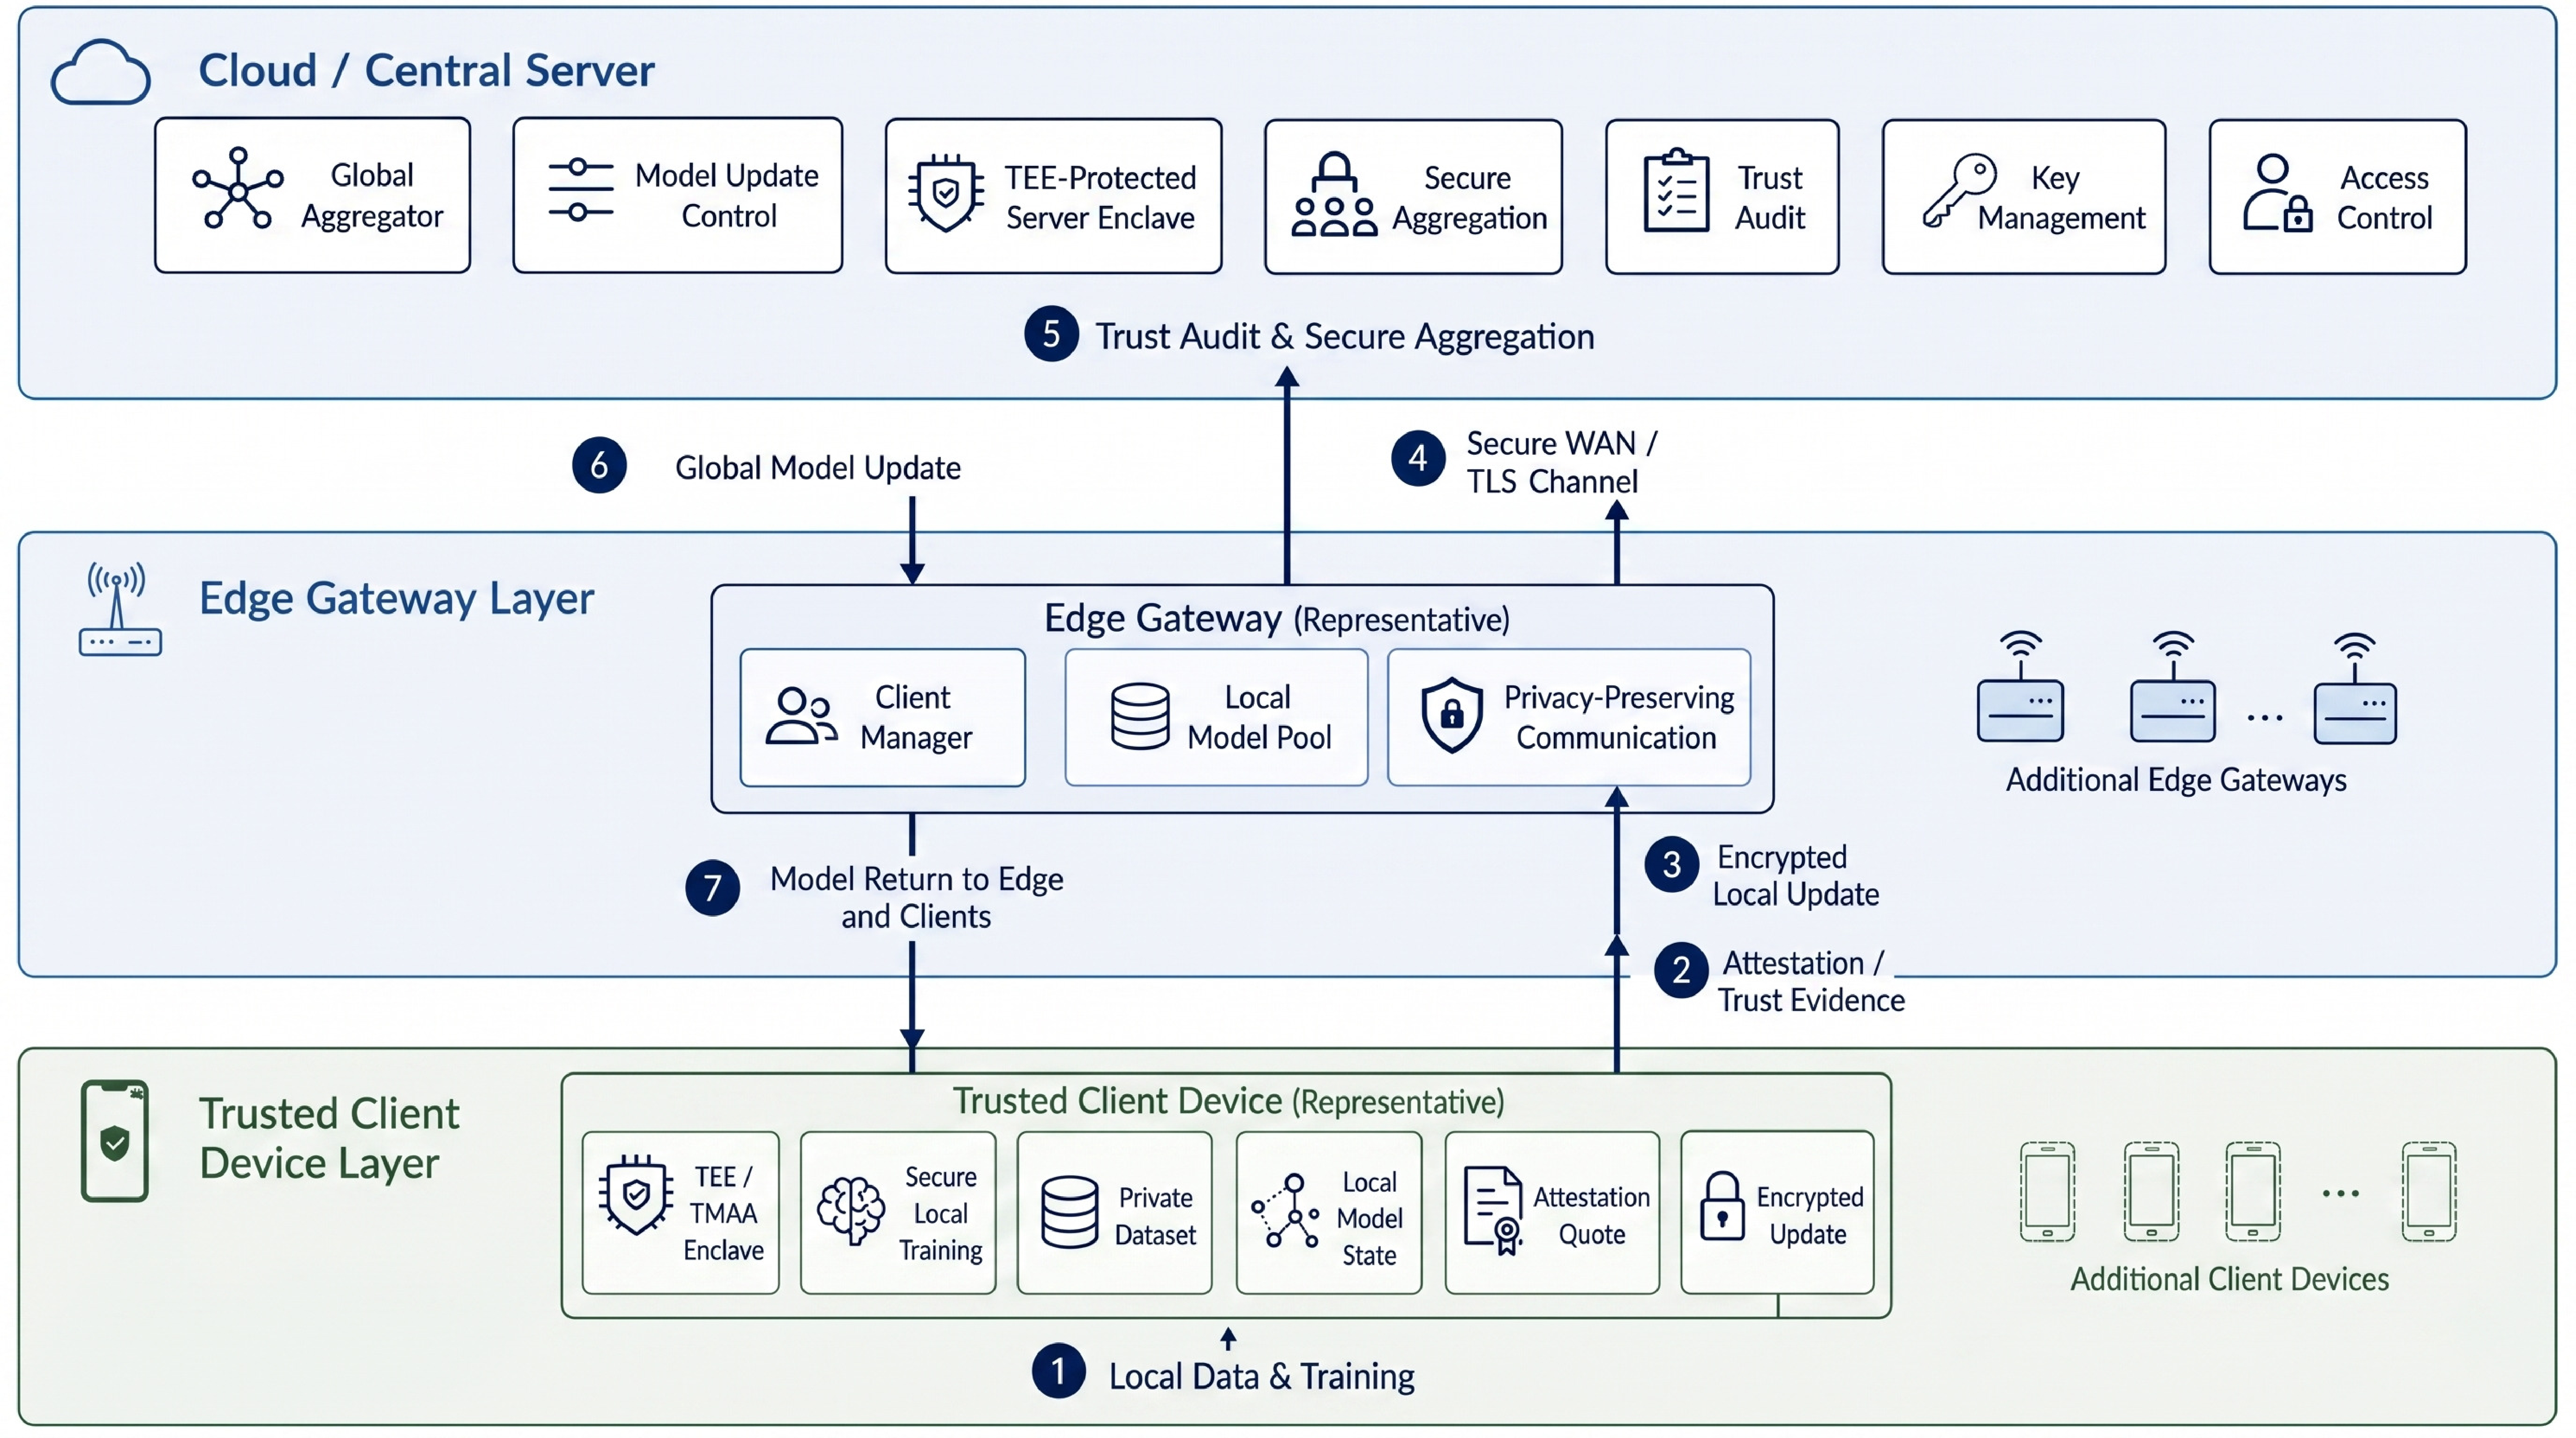
\includegraphics[width=0.84\textwidth]{fig1_system_arch.pdf}
    \caption{TEE 锚定的端-边-云协同架构。}
    \label{fig:system_arch}
\end{figure}

\begin{figure}[t]
    \centering
    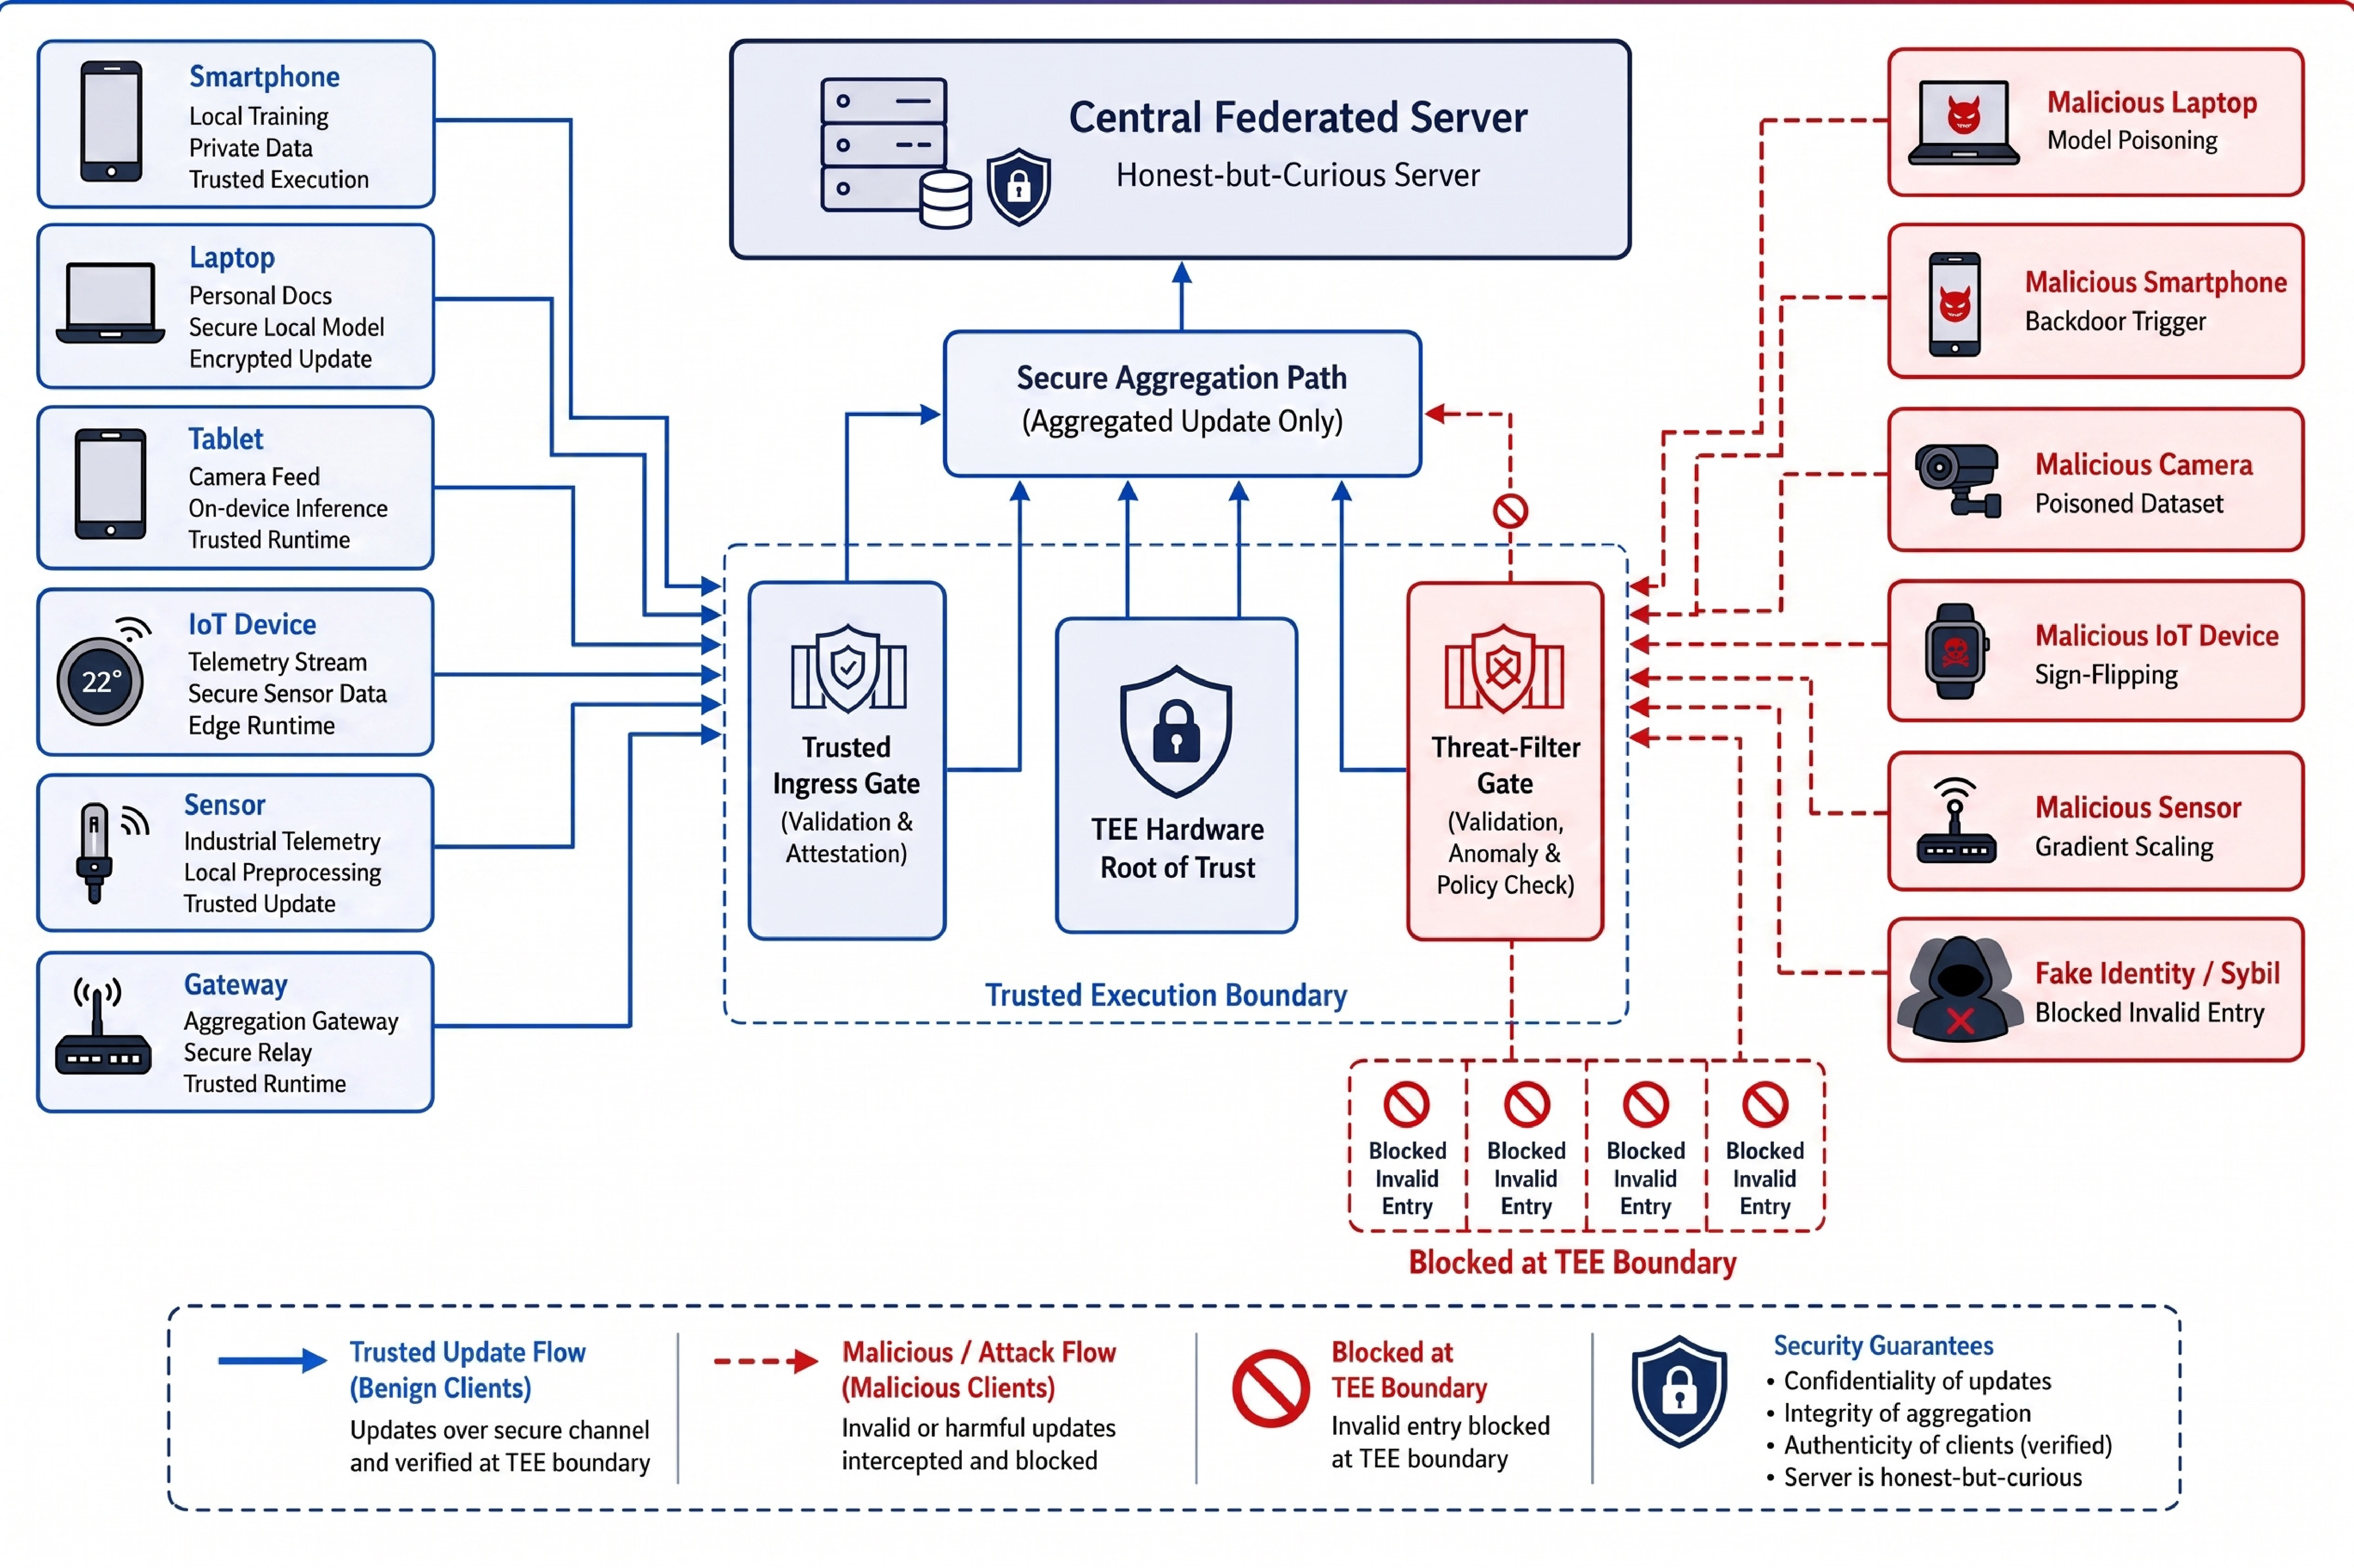
\includegraphics[width=0.80\textwidth]{fig2_threat_model.pdf}
    \caption{复合投毒与渗透威胁模型。}
    \label{fig:threat_model}
\end{figure}

\textbf{威胁模型。} 服务器遵循聚合协议，但属于诚实且好奇的观察者；它可以看到单个更新和审查统计量，但不能修改本文规定的状态转移规则。已准入客户端可以控制本地标签、样本或优化目标，并实施标签翻转、触发器后门、干净标签投毒、语义后门、符号翻转或梯度缩放。信任边界被明确限定为：TEE 保护证明关键代码、设备密钥、报告完整性、报告新鲜度以及更新绑定，使其免受受攻陷宿主系统的篡改，但不认证数据标签、样本、优化目标或语义意图。因此，攻击者可以在有效测量的训练流程内部执行数据级或目标级投毒。隐私感知验证层在不暴露原始样本的前提下检查选定的声明统计量，云端内容与时序审查则处理执行完整性无法决定的模型级影响。报告或更新绑定检查失败时，服务器在准入阶段拒绝该更新；有效报告并不意味着更新是良性的。物理探测和高级微架构侧信道不在威胁模型内。分析假设恶意准入客户端少于 50\%；50\% 实验是超出假设范围的压力测试，不构成 Byzantine 阈值或理论保证。服务器持有的 clean proxy set 用作内容审查的参考初始化；当服务器没有 proxy 时，由可信对等客户端分支执行对应参考操作。

\textbf{设计目标。} Trust Flow 旨在在给定攻击下保持收敛，限制长尾客户端的永久误封，并保持清晰的保证边界。执行证据、隐私感知统计证据、当前内容证据、历史效用和当前风险在按层聚合前始终保留各自含义。附加 TrustReport 约为 15 KB，服务器聚合与审查时间由 2.10 s 增至 4.85 s，辅助安全路径实测为每个准入客户端每轮约 11 ms，设备侧 TEE Quote 生成、签名和轻量监测另行实测为每个准入客户端每轮约 12--15 ms。本文按系统边界拆分开销，分别报告通信、证明、隐私感知验证和云端审查成本。

\section{Trust-Flow 框架}

Trust Flow 将每一轮 FL 划分为四个相互连接的阶段：准入与运行时信任评估、基于参考的内容审查、双流状态演化以及风险门控分层聚合。图~\ref{fig:framework} 展示了完整防御闭环。

\begin{figure}[t]
    \centering
    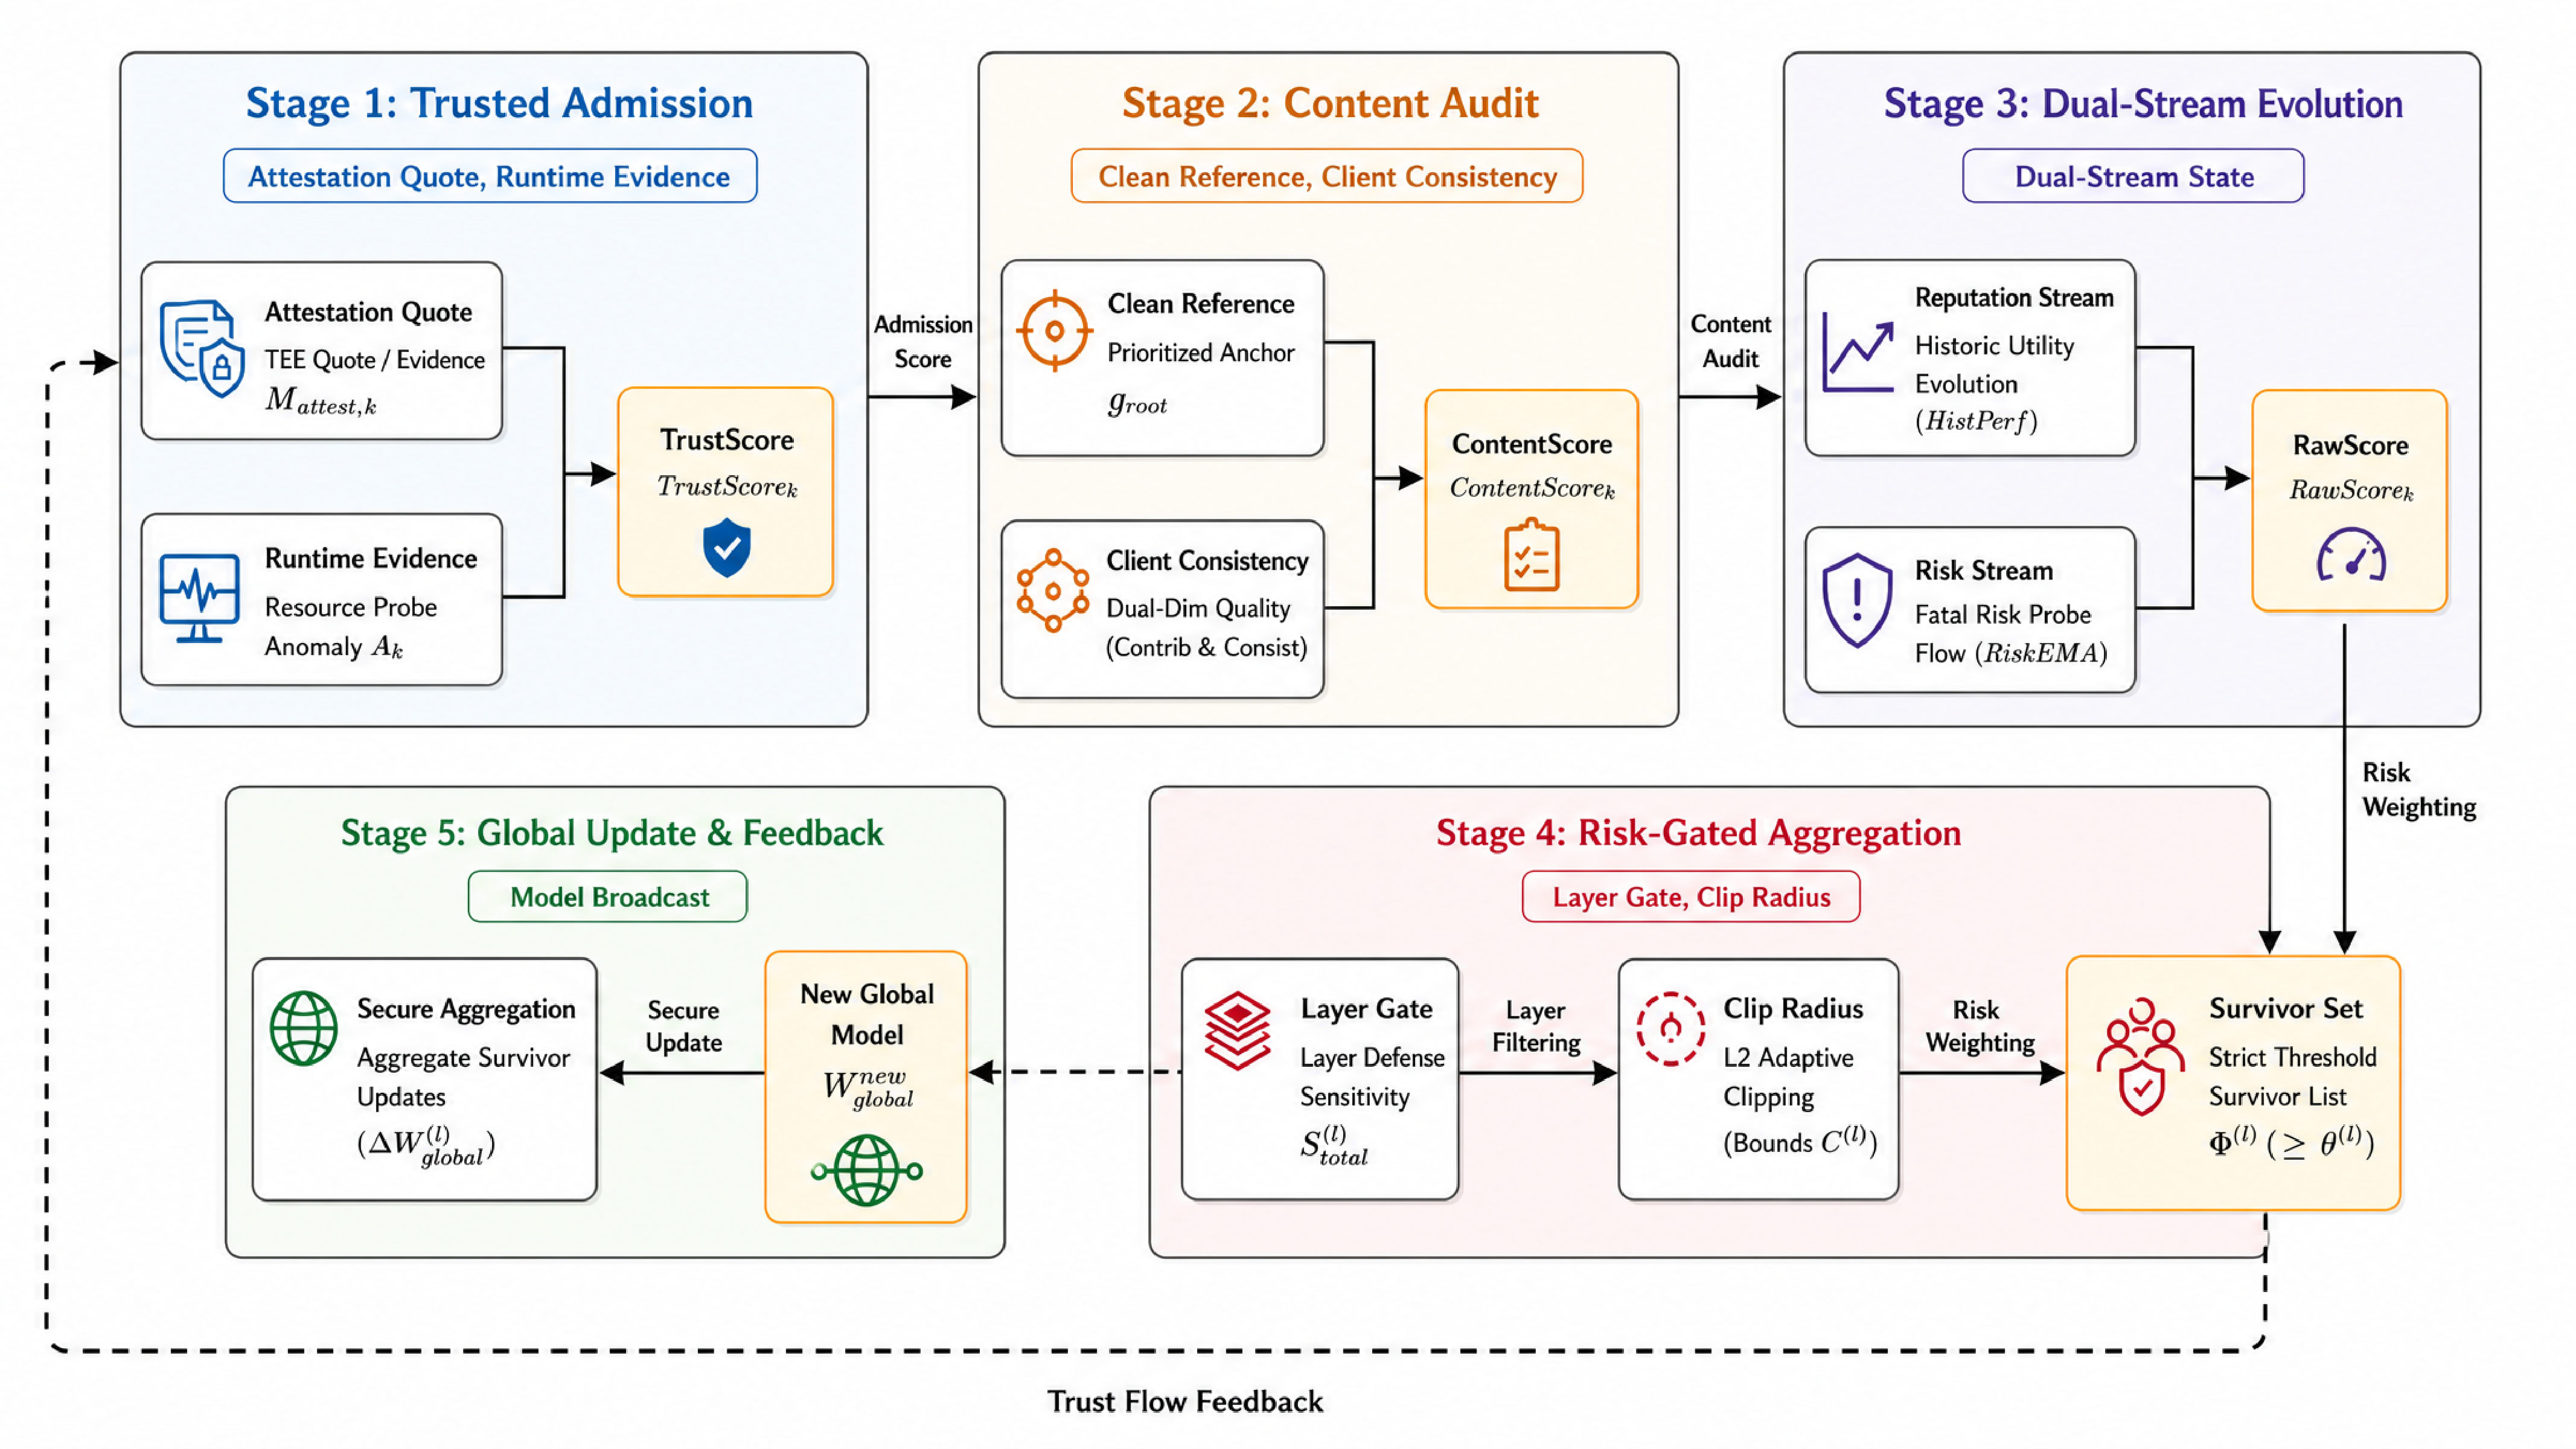
\includegraphics[width=0.86\textwidth]{fig3_arch.pdf}
    \caption{四阶段信任流防御闭环概览。}
    \label{fig:framework}
\end{figure}

四个阶段分别输出 $TrustScore$、$ContentScore$、慢速的 $HistPerf$/快速的 $RiskEMA$ 状态以及最终的 $RawScore$。无效证明首先被拒绝；随后审查隐私感知统计量与当前更新，更新时序状态，再分配分层权限。冷启动也遵循同一顺序：新客户端获得临时首轮权限，当前证据可以降低该权限，而不可逆状态转换需要累积证据。因此，单轮较低的内容分数对 Non-IID 客户端仍可恢复，而持续或当前强风险可以限制对应更新。



\subsection{准入与内容审查}

每个准入客户端都必须通过 TEE 式准入检查。令 $M_{\mathrm{attest},k}\in\{0,1\}$ 表示证明报告、随机数新鲜度以及轮次和更新摘要绑定是否有效。初始化期间，客户端调用设备唯一密钥并生成包含代码度量、运行配置、轮次随机数、更新摘要和单调新鲜计数器的远程证明 quote。只有通过该检查的客户端才获得通信权限。本地训练期间，可信管理代理监测行为序列 $\mathcal{X}_k^{(t)}=\{\Delta\mathrm{grad},\Delta\mathrm{loss},\mathrm{instr\_dist}\}$。将标准化特征直方图拼接后，令 $h_k^{(t)}=H(\mathcal{X}_k^{(t)})/H_{\max}\in[0,1]$，并定义
\begin{equation}
    R_k^{(t)}=\exp(\lambda h_k^{(t)}),\qquad
    Z_k^{(t)}=\operatorname{clip}\!\left(w_aM_{\mathrm{attest},k}+(1-w_a)(1-h_k^{(t)}),0,1\right),
\end{equation}
其中 $w_a=0.7$、$\lambda=1.0$。高熵只表示证据不确定性增加，并不直接等价于恶意标签。

标量 Kalman 递推为
\begin{equation}
    T_k^{-,(t)}=T_k^{(t-1)},\qquad P_k^{-,(t)}=P_k^{(t-1)}+Q,
\end{equation}
\begin{equation}
\begin{aligned}
    K_k^{(t)}&=\frac{P_k^{-,(t)}}{P_k^{-,(t)}+R_k^{(t)}},\\
    T_k^{(t)}&=T_k^{-,(t)}+K_k^{(t)}(Z_k^{(t)}-T_k^{-,(t)}),\\
    P_k^{(t)}&=(1-K_k^{(t)})P_k^{-,(t)}.
\end{aligned}
\end{equation}
其中 $Q=0.01$ 为固定过程噪声方差。新准入客户端初始化为 $T_k^{(0)}=1$、$P_k^{(0)}=0.25$ 和 $RiskEMA_k^{(0)}=0$，其准入权限为
\begin{equation}
    TrustScore_k^{(t)}=M_{\mathrm{attest},k}\operatorname{clip}\!\left(\frac{T_k^{(t)}}{1+P_k^{(t)}},0,1\right).
\end{equation}
高熵会降低 Kalman 增益，防止不确定观测突然改写跨轮信任。有效证明后的新客户端从 NORMAL 状态开始，首轮证据只能降低当前更新权限，不能触发不可逆黑名单。

    随后，服务器构造指导方向。若存在小型干净验证梯度，则 $g_{root}=g_{root\_clean}$；否则，使用高信任且上一轮风险较低的客户端，并以 $\omega_k^{ref}=TrustScore_k(1-RiskEMA_k^{prev})^2$ 作为参考权重。实验中服务器持有均衡的 500 张 proxy 样本（CIFAR-10 每类 50 张），该集合不参与客户端训练。固定 proxy 划分属于共同实验协议；具有参考通道的方法使用它执行各自定义的参考操作，没有该通道的方法在相同数据、初始化和通信预算下保留自身聚合规则。proxy 为内容审查提供稳定的指导种子，初始化之后仍由对等一致性和时序状态持续提供证据；当没有 proxy 时，由可信对等客户端分支构造相应参考。对每个客户端更新，内容质量由参考一致性和群体一致性共同构成：
\begin{align}
    S_{contrib,k}  & =\max(0,\alpha_1+\alpha_2\cos(\Delta W_k,g_{root})),                                  \\
    S_{consist,k}  & =\frac{\sum_{j\ne k}TrustScore_j\max(0,\alpha_1+\alpha_2\cos(\Delta W_k,\Delta W_j))}
    {\sum_{j\ne k}TrustScore_j+\varepsilon},                                                               \\
    ContentScore_k & =\frac{(1+\beta_{fusion}^2)S_{consist,k}S_{contrib,k}}
    {\beta_{fusion}^2S_{consist,k}+S_{contrib,k}+\varepsilon}.
\end{align}
其中 $\beta_{fusion}>1$ 会提高干净方向的影响，有助于抵抗合谋漂移。这里采用调和式融合并非只为数值平滑，而是要求客户端同时在干净参考和可信群体两个方向上都具有合理性。仅有较高群体一致性不足以抵抗合谋，只有较高参考一致性又可能过度惩罚合法 Non-IID 更新。

\subsection{双流状态演化}

单一信誉分会混淆由数据偏斜导致的低效用和由攻击导致的高风险。Trust Flow 因此将客户端状态分为历史效用流和瞬时风险流。令 $q_k^{(t)}=\operatorname{clip}(ContentScore_k^{(t)},0,1)$，历史流使用显式衰减 Beta 更新：
\begin{equation}
    a_k^{(t)}=\beta_h a_k^{(t-1)}+q_k^{(t)},\quad
    b_k^{(t)}=\beta_h b_k^{(t-1)}+1-q_k^{(t)},\quad
    HistPerf_k^{(t)}=\frac{a_k^{(t)}}{a_k^{(t)}+b_k^{(t)}+\varepsilon}.
\end{equation}
新客户端从 $a_k^{(0)}=b_k^{(0)}=1$ 开始，因此 $HistPerf_k^{(0)}=0.5$；衰减因子 $\beta_h\in(0,1)$ 在测试前固定。首轮中，有效准入客户端保持 NORMAL，并根据当前内容和风险获得临时权限。首轮证据记录到下一次状态更新，不能单独触发不可逆黑名单；临时权重提供即时控制，而永久决策依赖跨轮证据。历史流缓慢调整权限，使低效用不直接导致移除；风险流采用
\begin{equation}
    RiskEMA_k^{(t)}=\beta_rRiskEMA_k^{(t-1)}+(1-\beta_r)Risk_k^{inst},
\end{equation}
其中 $Risk_k^{inst}$ 为当轮最大探针，因此强警告不会被良性历史行为平均掉。

有效证明后的新客户端从 NORMAL 状态开始。令 $u_k^{(t)}=1-HistPerf_k^{(t)}$、$r_k^{(t)}=RiskEMA_k^{(t)}$，阈值 $(\tau_h,\tau_s,\tau_q,\tau_b)=(0.26,0.64,0.80,0.90)$ 分别表示效用缺口、软风险、隔离和黑名单。NORMAL 客户端在连续两轮满足 $u_k^{(t)}>\tau_h$ 或 $r_k^{(t)}\geq\tau_s$ 后进入 SUSPECT；SUSPECT 客户端在连续三轮满足相同条件，或某一轮当前探针满足 $Risk_k^{inst}\geq\tau_q$ 后进入 QUARANTINE；QUARANTINE 客户端在连续四轮满足 $r_k^{(t)}\geq\tau_b$ 后进入 BLACKLIST。SUSPECT 或 QUARANTINE 恢复需要连续两轮满足 $u_k^{(t)}\leq\tau_h$ 且 $r_k^{(t)}<\tau_s$；BLACKLIST 在一次实验内不可逆。条件不满足时计数器重置，状态更新在分层聚合前完成。首轮控制与永久准入决策具有不同含义：前者限制当轮贡献，后者需要持续证据。

这两个流只在计算聚合权限时汇合：
\begin{align}
    RawScore_k^{(t)} & = (TrustScore_k^{(t)})^\alpha(ContentScore_k^{(t)})^\beta
    (HistPerf_k^{(t)})^\gamma \nonumber \\
               & \quad \times (1-RiskEMA_k^{(t)})^p .
\end{align}
因此，当轮风险可以否决高历史信誉的潜伏攻击，而低相似度的良性长尾客户端仍可通过慢速流恢复。

\begin{figure}[t]
    \centering
    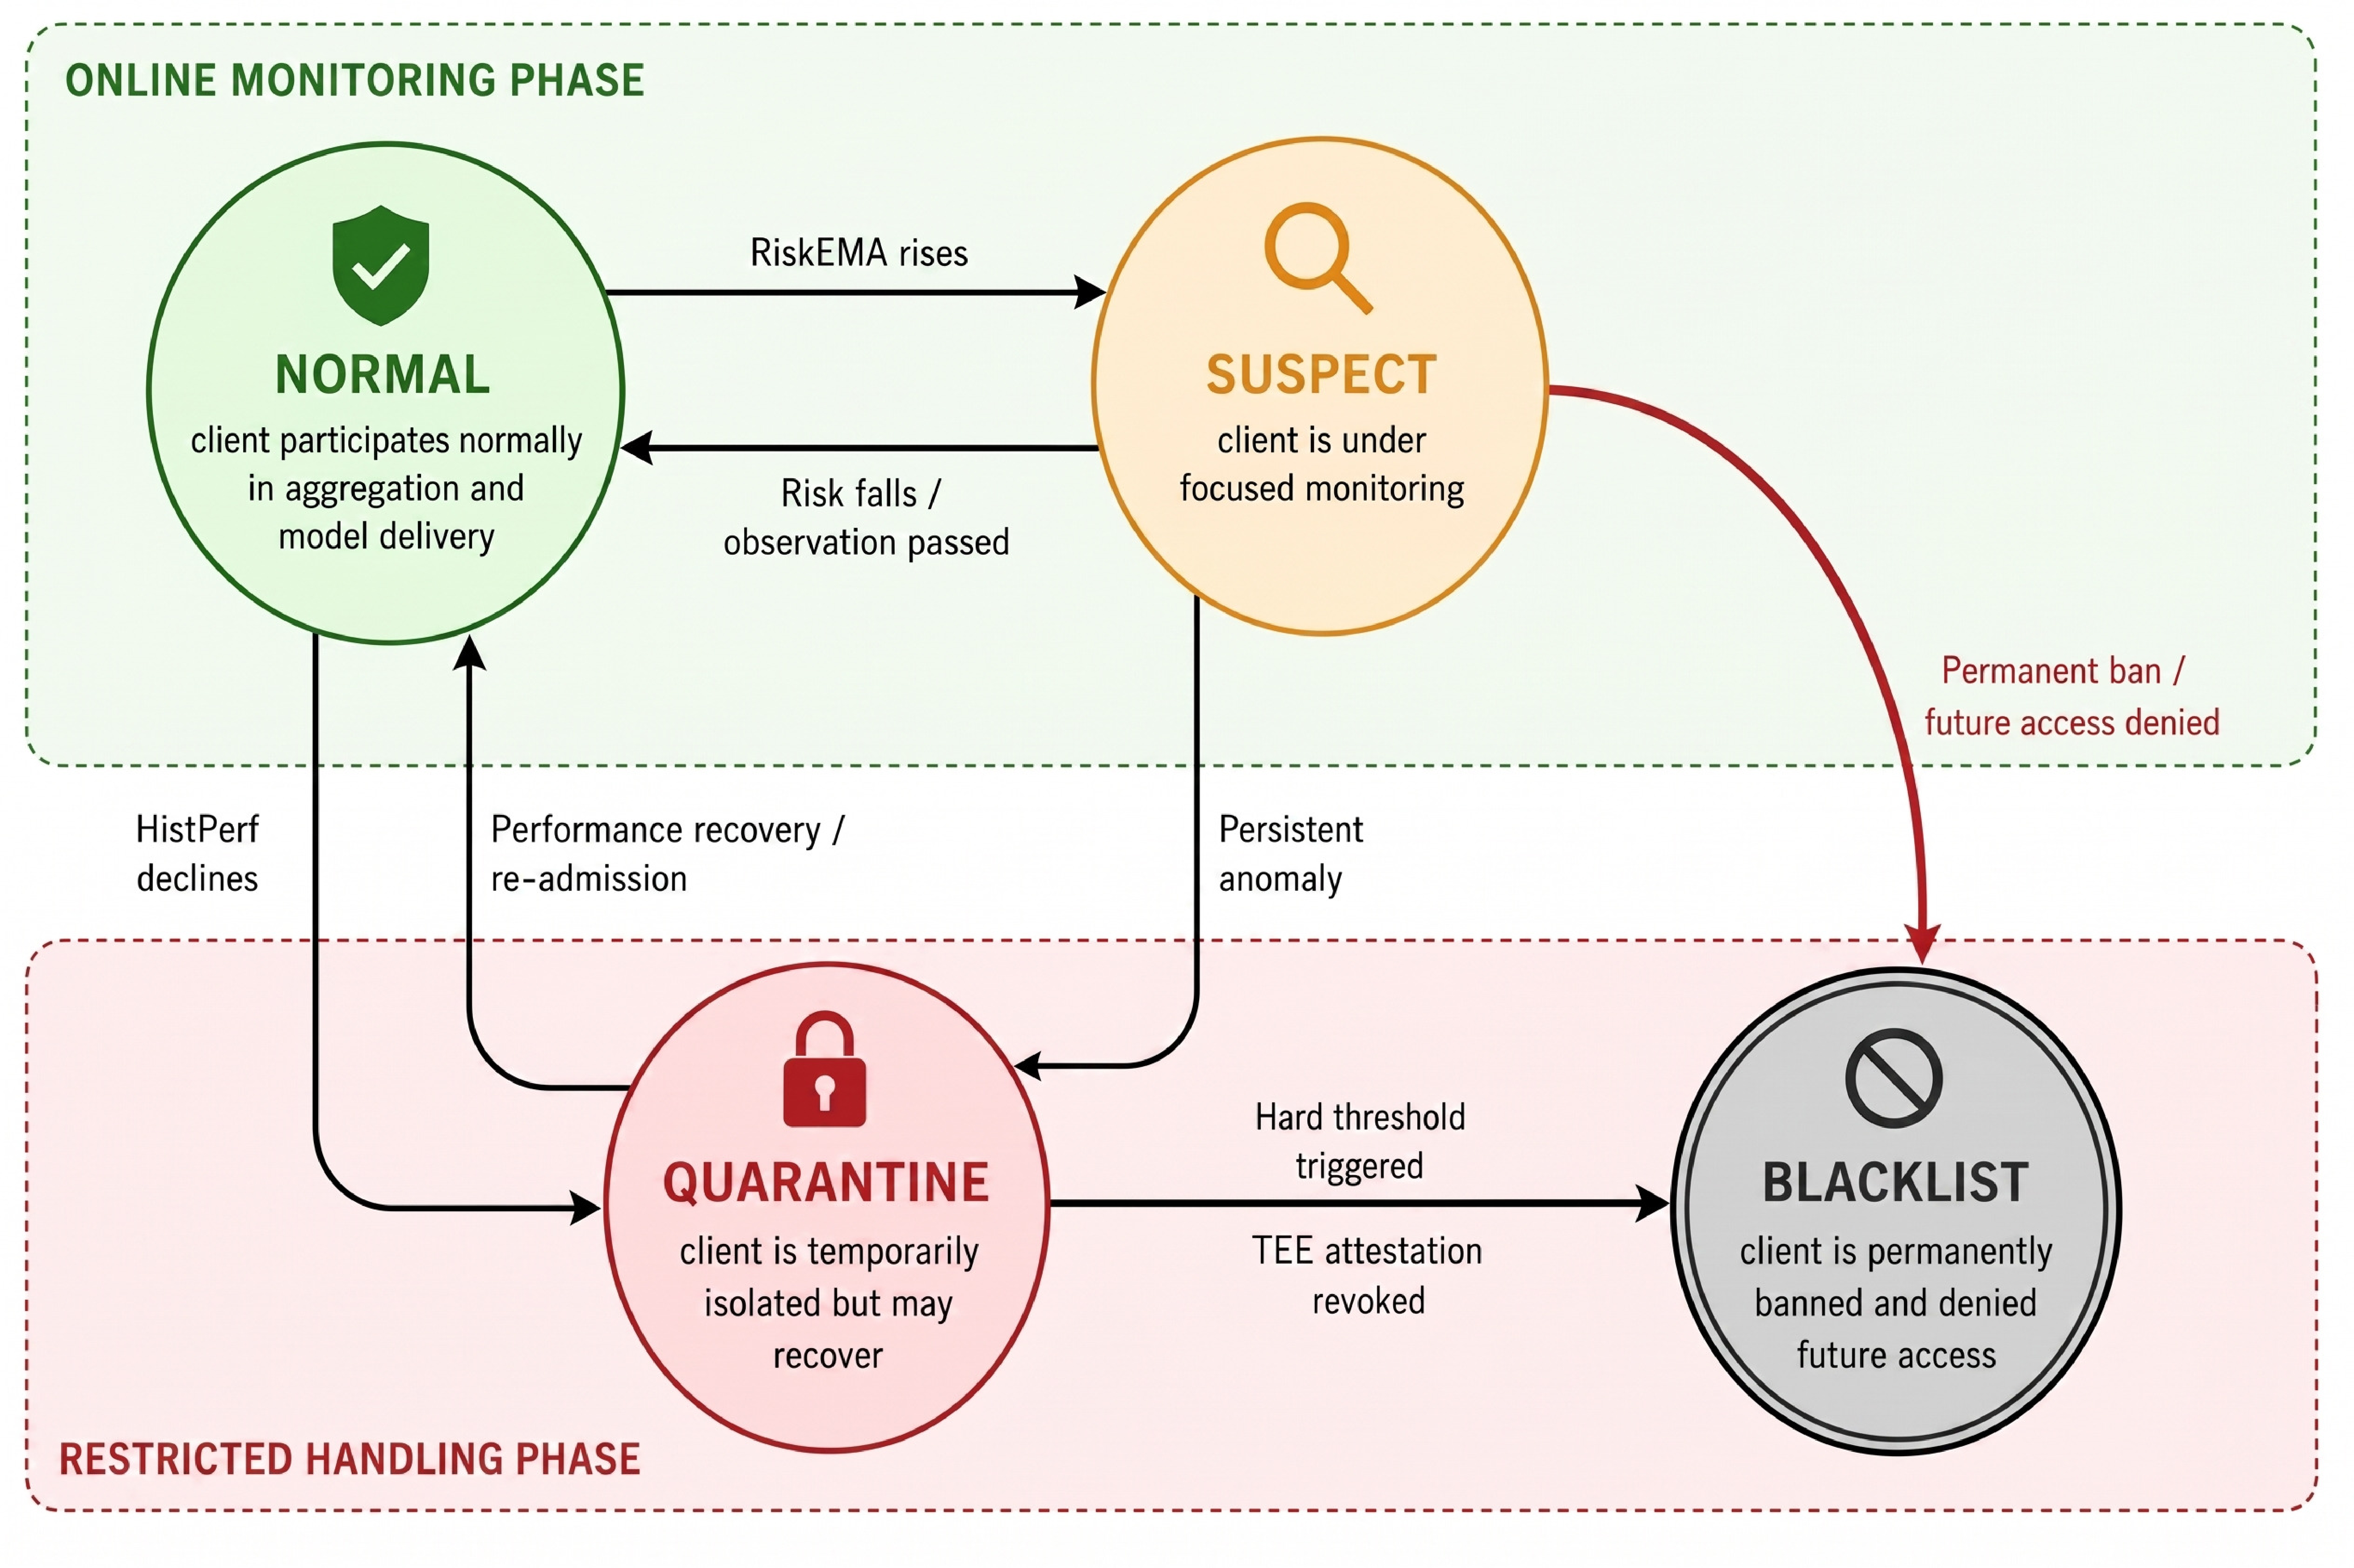
\includegraphics[width=0.76\textwidth]{fig4_state.pdf}
    \caption{由历史效用和短期风险驱动的客户端状态转换自动机。}
    \label{fig:state_machine}
\end{figure}

\subsection{风险门控分层聚合}

后门往往集中在深层，而浅层特征层可能携带有价值的异构信息。Trust Flow 因此为每个层 $l$ 分配敏感度分数：
\begin{figure}[t]
    \centering
    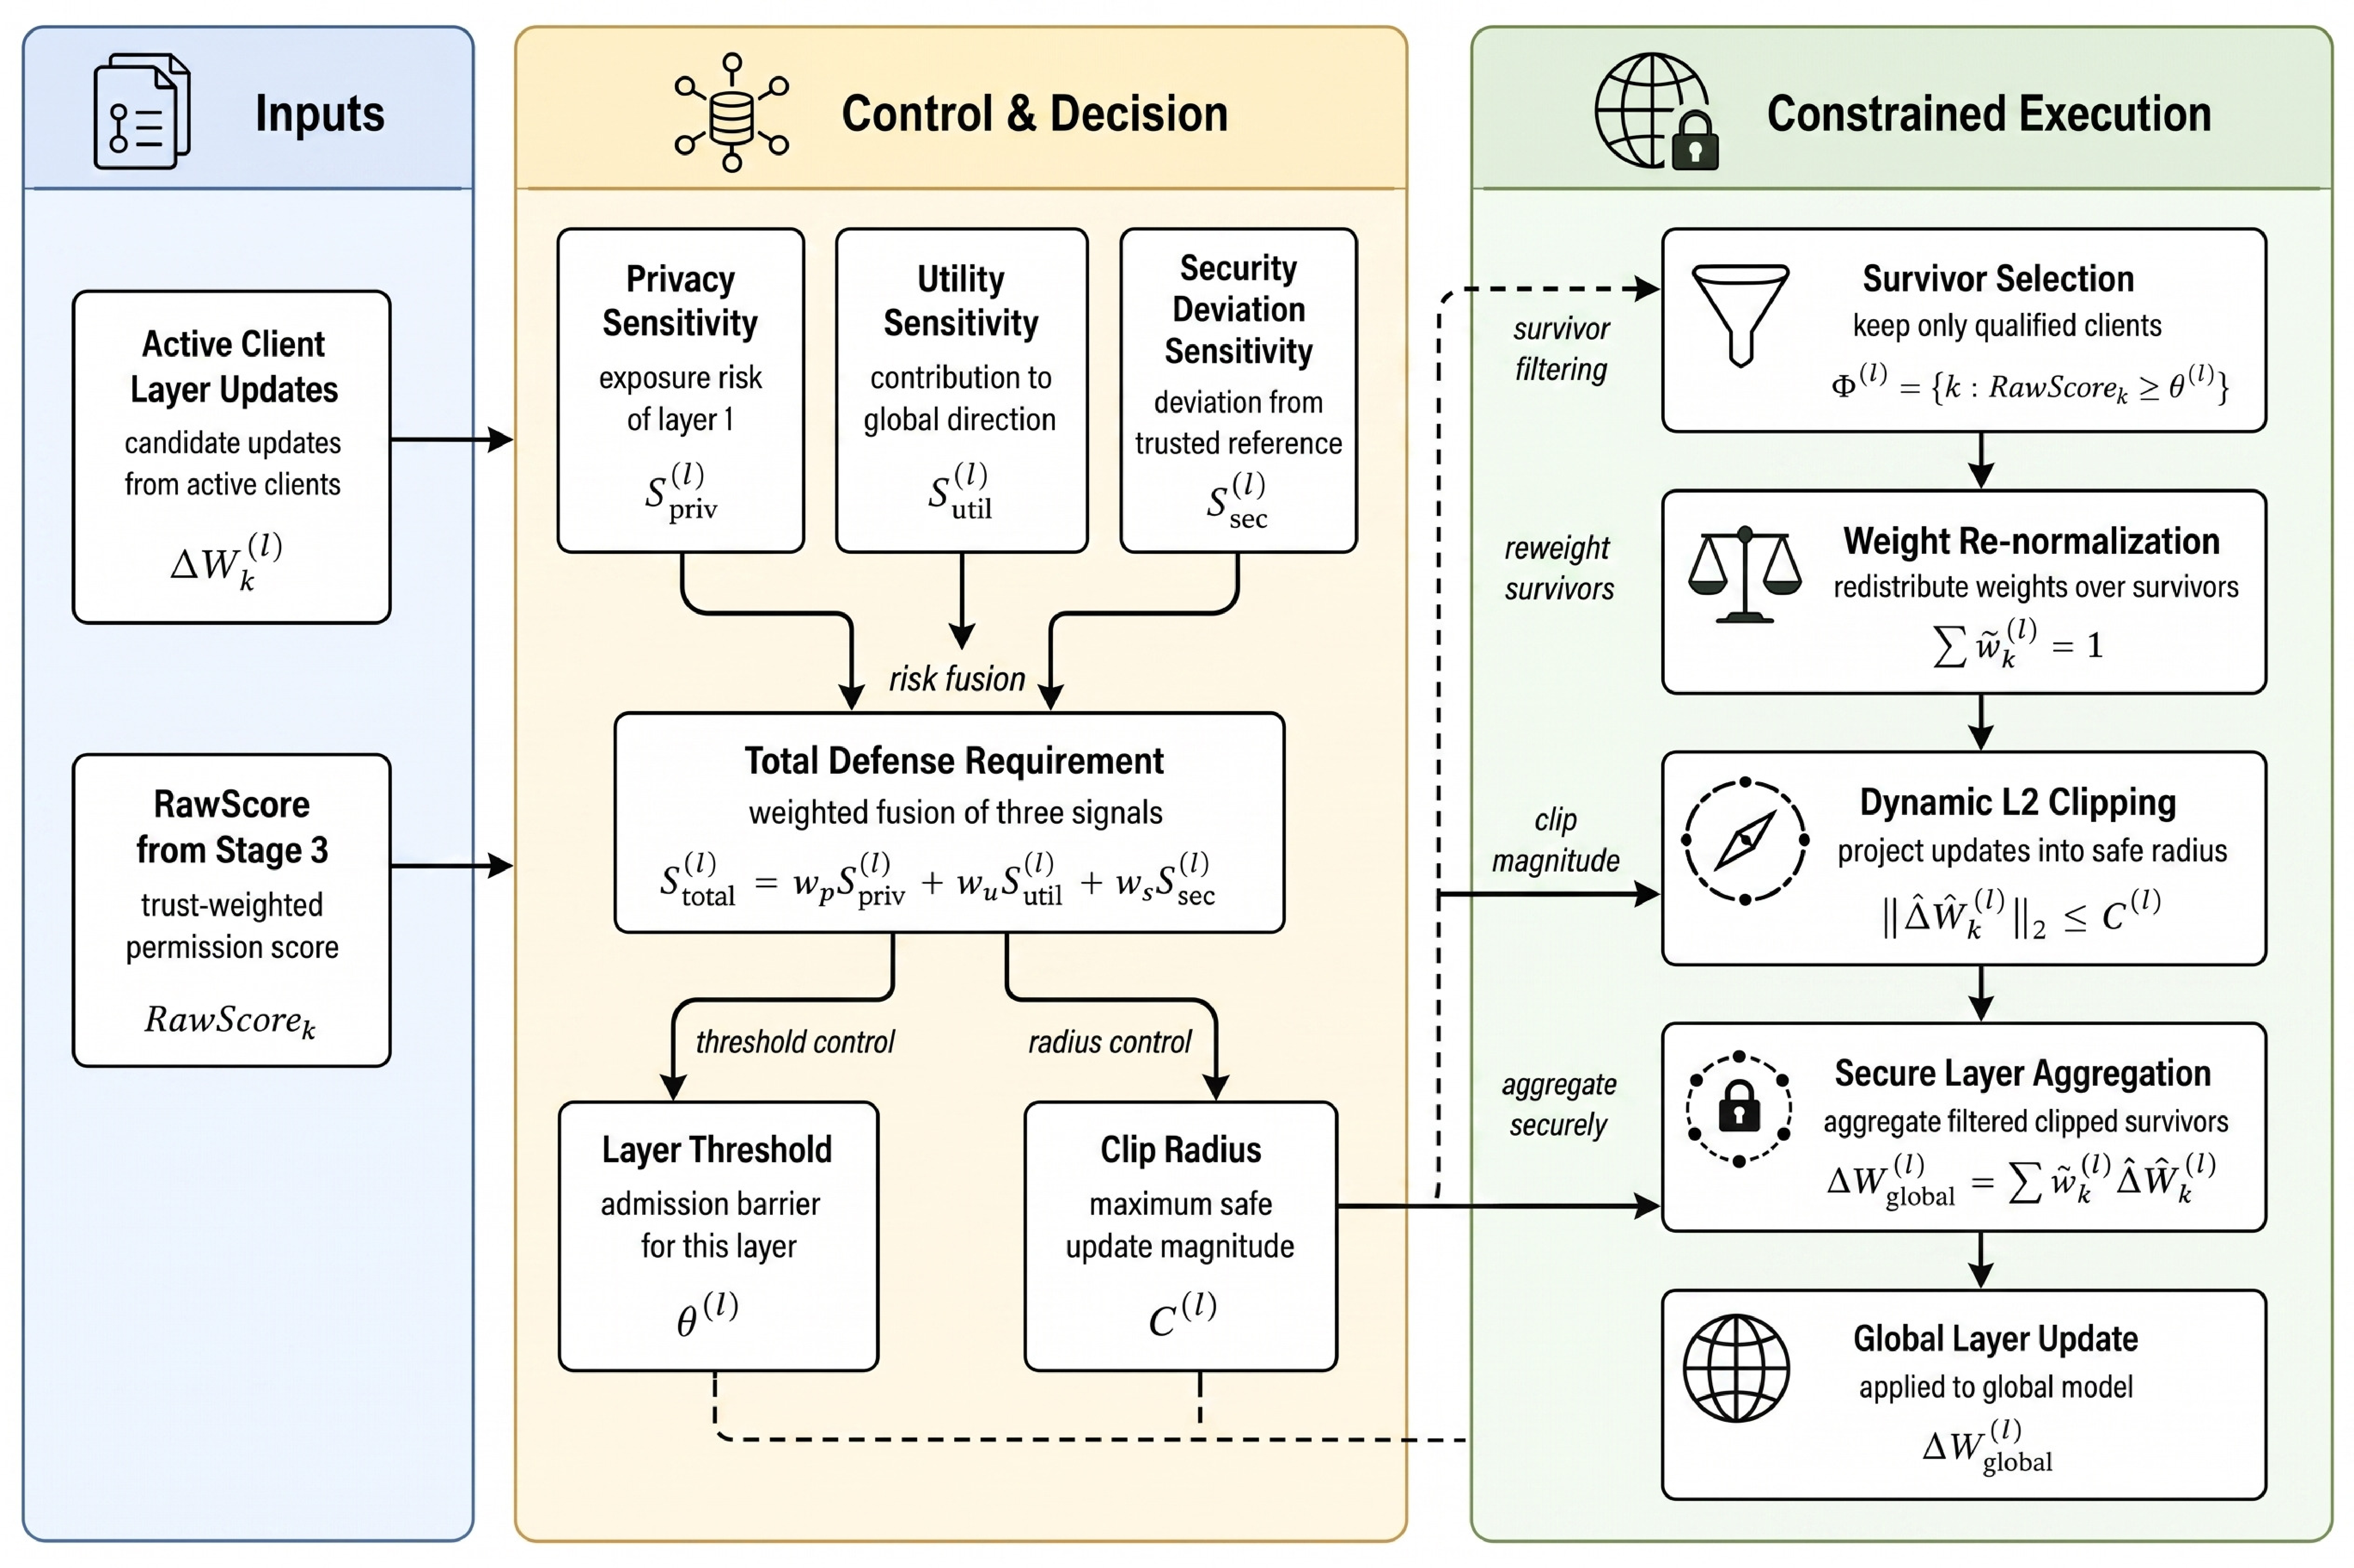
\includegraphics[width=0.78\textwidth]{fig5_layer.pdf}
    \caption{风险门控的按层裁剪与差异化聚合。}
    \label{fig:layer_gating}
\end{figure}
定义三个归一化分量：
\begin{align}
    S_{priv}^{(l)}&=\exp(-\tau_p l/L),\qquad
    S_{util}^{(l)}=\frac{\|g_{root}^{(l)}\|_2}{\max_m\|g_{root}^{(m)}\|_2+\varepsilon},\\
    S_{sec}^{(l)}&=\frac{1}{2}\left(1-\frac{1}{|\mathcal{T}|}
    \sum_{k\in\mathcal{T}}\cos(\Delta W_k^{(l)},g_{root}^{(l)})\right),
\end{align}
其中 $\mathcal{T}=\{k\in\mathcal{A}:M_{\mathrm{attest},k}=1,\,RiskEMA_k^{(t-1)}<\tau_s\}$ 为可信参考集；若该集合为空，服务器仅使用 $\mathcal{A}$ 进行归一化并记录没有可信对等参考。因此 $S_{priv}^{(l)}$、$1-S_{util}^{(l)}$ 和 $S_{sec}^{(l)}$ 均位于 $[0,1]$。取
\begin{equation}
    S_{total}^{(l)}=w_pS_{priv}^{(l)}+w_u(1-S_{util}^{(l)})+w_sS_{sec}^{(l)},\quad
    (w_p,w_u,w_s)=(0.3,0.3,0.4),
\end{equation}
并设置 $\theta^{(l)}=\mu_{base}+\lambda_sS_{total}^{(l)}$ 与 $C^{(l)}=C_{base}/(S_{total}^{(l)}+\varepsilon_c)$。若某层出现更强可疑漂移，该层会变得更难进入且裁剪更紧；若某层仍稳定接近参考方向，则保留更多良性异构容量。

设置 $\tau_p=3.0$、$\varepsilon=\varepsilon_c=10^{-8}$，并将 $C_{base}$ 定义为分层门控前可信客户端更新范数的中位数。这些设置使敏感度项无量纲，并使裁剪尺度适应当轮更新幅度。

幸存者集合为 $\Phi^{(l)}=\{k\in\mathcal{A}\mid RawScore_k^{(t)}\geq\theta^{(l)}\}$，并保留原始数据量权重 $p_k$，其权重重新归一化为
\begin{equation}
    \tilde{w}_{k}^{(l)}=\frac{p_kRawScore_k^{(t)}}{\sum_{j\in\Phi^{(l)}}p_jRawScore_j^{(t)}+\varepsilon},\quad
    \widehat{\Delta W}_k^{(l)}=\frac{\Delta W_k^{(l)}}{\max(1,\|\Delta W_k^{(l)}\|_2/C^{(l)})}.
\end{equation}
最终更新为 $\Delta W_{global}^{(l)}=\sum_{k\in\Phi^{(l)}}\tilde{w}_{k}^{(l)}\widehat{\Delta W}_k^{(l)}$。若 $\Phi^{(l)}=\varnothing$，则保留 $RawScore$ 最大的客户端并赋予单位归一化权重，同时仍执行该层裁剪。权重重归一化可以防止剔除风险客户端后有效学习率缩小。

这种按层控制旨在保留有用的浅层表征，同时加固攻击敏感度更高的层。以语义后门为例，攻击通常更集中地改变最终分类层或深层特征层；统一全局裁剪要么足够宽松以保留浅层特征，要么足够严格以压制深层攻击，却很难兼顾二者。Trust Flow 允许不同层在同一轮采用不同策略：深层可以拒绝低权限客户端并收紧更新半径，浅层在参考一致性稳定时仍可保持较宽松阈值。这种差异化处理很重要，因为统一裁剪半径会过度压制良性特征提取层，并在恶意客户端已被移出幸存集后拖慢收敛。

重归一化步骤对收敛同样关键。若没有该步骤，剔除可疑客户端会降低有效聚合权重之和，并形成隐式学习率衰减。这种衰减容易被误认为是鲁棒性控制带来的正常副作用，但在固定 30 轮训练预算下会直接拖慢优化。Trust Flow 因此将过滤与优化视为耦合操作：移除不安全权重后，剩余可信权重会先被投影回有效聚合单纯形，再进入裁剪和分层组装。

\subsection{风险探针计算}

短期风险流使用互为补充的探针，而不由任一探针独立作出最终裁决。第 $t$ 轮中，客户端 $k$ 的归一化通道定义为
\begin{align}
 r_{grad,k}^{(t)}&=\operatorname{clip}\!\left(\frac{1-\cos(\Delta W_k,g_{root})}{2},0,1\right),\\
 r_{amp,k}^{(t)}&=\operatorname{clip}\!\left(\frac{\|\Delta W_k\|_2}{\operatorname{median}_j\|\Delta W_j\|_2+\varepsilon}-1,0,1\right),\\
 r_{clean,k}^{(t)}&=\operatorname{clip}\!\left(\frac{\mathcal{L}_{probe}(W+\Delta W_k)-\mathcal{L}_{probe}(W)}{\delta_{clean}+\varepsilon},0,1\right),\\
 r_{trigger,k}^{(t)}&=\operatorname{clip}\!\left(\frac{\mathrm{KL}(\mathcal{H}(A_{base})\|\mathcal{H}(A_k))}{\delta_{trigger}+\varepsilon},0,1\right),\\
 \bar c_k^{(t)}&=\frac{\sum_{j\ne k}TrustScore_j\,c_{kj}}{\sum_{j\ne k}TrustScore_j+\varepsilon},\quad
 r_{peer,k}^{(t)}=\operatorname{clip}(1-\bar c_k^{(t)},0,1),
\end{align}

其中 $c_{kj}=\cos(\Delta W_k,\Delta W_j)$。对于触发器探针，$A_{base}$ 为当前全局模型在服务器 proxy 集上的激活直方图，$A_k$ 为应用候选更新后的对应直方图。采用最后一个卷积块与分类器前表示的 32 区间直方图。每轮中，$\delta_{clean}$ 与 $\delta_{trigger}$ 由可信集合 $\mathcal{T}$ 上相应值的中位数加三倍中位绝对偏差确定，使校准独立于待测候选。定义 $Risk_k^{inst}=\max\{1-M_{\text{attest},k},r_{grad,k},r_{amp,k},r_{clean,k},r_{trigger,k},r_{peer,k}\}$。

最大值规则保留互补警告：方向与幅度通道揭示参数攻击，干净损失与激活通道针对更隐蔽的后门。对等分歧作为辅助证据，因为合法长尾更新也可能偏离多数方向。执行顺序为参考构造、当前更新审查、状态更新、分层聚合。

\subsection{保证组合与参考数据作用}

四类证据承担互补职责。证明与隐私感知验证确定声明的执行过程和选定统计量是否满足准入策略，但不认证本地目标的语义意图。云端审查利用可用参考或对等证据检查提交更新及其行为，时序状态则决定一次异常是暂时现象还是持续行为。这种组合避免仅因更新带有有效签名就接受执行有效但语义有害的更新，也避免仅因一次低相似度观测就永久移除合法长尾客户端。

干净 proxy 是参考初始化和校准来源，而不是信任流的替代物。小型服务器参考集可用时，它提供稳定方向和共同探针接口；没有服务器 proxy 时，对等参考分支保留相同的内容与时序决策顺序。两种分支的最终决策均来自更新证据、状态转换和分层聚合规则，不将单次参考观测直接视为恶意标签。

\section{实验}

\subsection{实验设置}

实验使用 Flower 1.5.0 与 PyTorch，在 CIFAR-10 上训练适配后的 ResNet-18：首层卷积为 $3\times3$、步长为 1，移除初始最大池化层，分类器输出 10 类。训练和可信执行在两个基于 Intel 与 AMD、支持 TEE 的真实平台上完成；NVIDIA A10 GPU 执行模型训练，CPU 侧 TEE 隔离证明、可信监测、报告生成和准入状态处理。软件栈为 Ubuntu 20.04.6 LTS 与 CUDA 12.8。50,000 张训练图像划分为一个对所有客户端复用的 5,000 张共享客户端池和 45,000 张专属图像：客户端 0--9 使用 IID 划分，客户端 10--14 使用 Dirichlet $\alpha=1.0$，客户端 15--19 使用 $\alpha=0.1$ 的强长尾划分。服务器另行持有从 CIFAR-10 留出参考划分中取得的 500 张均衡 proxy 样本（每类 50 张），该集合与客户端训练和最终评测数据不相交。所有方法共享固定 proxy 划分与初始化；依赖参考的方法将其用于各自定义的指导操作和探针，没有参考通道的方法保留标准聚合规则。所有方法采用相同优化器、通信预算、客户端划分和初始模型。

正式 30\% 攻击设置包含六个恶意客户端：Client 0 执行 $\gamma=0.5$ 的无目标标签翻转；Client 1 在 20\% 样本中注入固定右下角 $3\times3$ 触发器并以类别 0 为目标；Client 2 在 20\% 样本上执行保持标签的干净标签扰动并使用相同目标；Client 3 在 20\% 样本上施加固定语义属性偏置并将偏置子集分配到类别 0；Client 4 执行无目标符号翻转；Client 5 将更新放大 100 倍。六类行为在每轮本地训练中同时激活。另有五个无有效证书的 Sybil 节点和三个伪造低工作负载的 free-rider 节点仅用于验证第一阶段门控，并在统计聚合前被拦截，因此后续指标均在 20 个准入客户端上计算。每次运行包含 30 轮和 3 个本地 epoch。聚合值在两个平台各 5 个种子的 10 个平台--种子运行上计算，节点状态轨迹使用每个平台一个固定种子。

每个平台运行 5 个独立种子，准确率和 ASR 的均值与标准差在 10 个平台--种子运行上计算。永久封禁 FPR 以被不可逆列入黑名单的良性客户端计算，临时 SUSPECT 或 QUARANTINE 状态被视为可恢复控制动作。节点轨迹图使用每个平台一个固定种子，聚合表格使用重复运行结果。所有方法采用相同客户端划分、初始模型、优化器、通信预算、攻击时序、参考数据可用性和 Non-IID 划分，并按照自身定义的决策规则使用共同证据。

对于每种目标攻击 $a\in\{\mathrm{trigger},\mathrm{clean},\mathrm{semantic}\}$，令 $\mathcal{B}_a$ 为携带相应触发器或属性的测试子集，$y_a^*$ 为声明的目标类别，定义 $ASR_a=|\{x\in\mathcal{B}_a:\arg\max f(x)=y_a^*\}|/|\mathcal{B}_a|$，主表报告宏平均 $ASR_{target}=\frac{1}{3}\sum_a ASR_a$。收敛轨迹分别保留三种攻击的 ASR。无目标标签翻转、符号翻转与缩放不计入该分子，而通过干净准确率、损失和状态转换时间评估。无状态基线没有对应的永久封禁状态，因此其 FPR 标为 N/A。

\begin{table}[t]
    \centering
    \caption{实验配置与主要超参数。}
    \label{tab:setup}
    \small
    \begin{tabular*}{\textwidth}{@{\extracolsep{\fill}} p{2.45cm} p{5.2cm} p{4.25cm}}
        \toprule
        类别 & 设置 & 取值 \\
        \midrule
        FL 任务 & 数据集/模型/准入客户端 & CIFAR-10/CIFAR-适配 ResNet-18/$K=20$ \\
        优化 & 本地 epoch、学习率、动量、轮次 & $3$, $0.001$, $0.9$, $30$ \\
        数据异构 & 共享客户端池、服务器 proxy、Group A/B/C & $5000$、$500$、$\alpha=1.0,0.1$ \\
        信任流 & $\alpha_1,\alpha_2,\beta_{fusion}$; $\beta_h,\beta_r$ & $0.6,0.4,2.0$; $0.9,0.85$ \\
        准入滤波 & $w_a,\lambda,Q$; $T_0,P_0,RiskEMA_0$ & $0.7,1.0,0.01$; $1,0.25,0$ \\
        分层门控 & 融合指数；$\mu_{base},\lambda_s$ & $3.0,1.0,0.5,1.0$; $0.4,1.2$ \\
        敏感度 & $\tau_p; w_p,w_u,w_s$ & $3.0; 0.3,0.3,0.4$ \\
        数值稳定性 & $\varepsilon,\varepsilon_c$; $C_{base}$ & $10^{-8},10^{-8}$; 可信范数中位数 \\
        状态机 & $\tau_h,\tau_s,\tau_q,\tau_b$; 持续轮数 & $0.26,0.64,0.80,0.90$; $2,3,4$ \\
        \bottomrule
    \end{tabular*}
\end{table}

\subsection{整体防御性能}

图~\ref{fig:main_results} 总结收敛、三类目标攻击的 ASR 轨迹、信任状态轨迹和特征可视化。给定的 30\% 混合攻击协议中，六类攻击在每个本地训练轮次同时激活，因此这是同时攻击测试，而非逐个攻击的汇总。Trust Flow 达到 92.31\% 干净准确率和 10.21\% 目标 ASR 宏平均，接近 CIFAR-10 十类任务的 10\% 随机目标命中率。客户端轨迹展示各保证层的协同作用：执行有效的客户端仍需接受语义审查，当前探针暴露有害更新行为，时序流判断观测是暂时还是持续。合法长尾节点可能受到临时限制而保留积累的历史，持续风险则可推动客户端经过定义的状态转换。这些观察描述给定协议及各比较方法使用的证据接口。

轨迹中，标签、触发器、语义、符号翻转与缩放攻击表现出持续风险；长尾正常客户端则可以在风险不持续时恢复。t-SNE 仅用于展示所得信任状态特征，定量结论来自准确率、ASR 和状态转换指标。

\begin{figure}[t]
    \centering
    \begin{minipage}{0.49\textwidth}
        \centering
        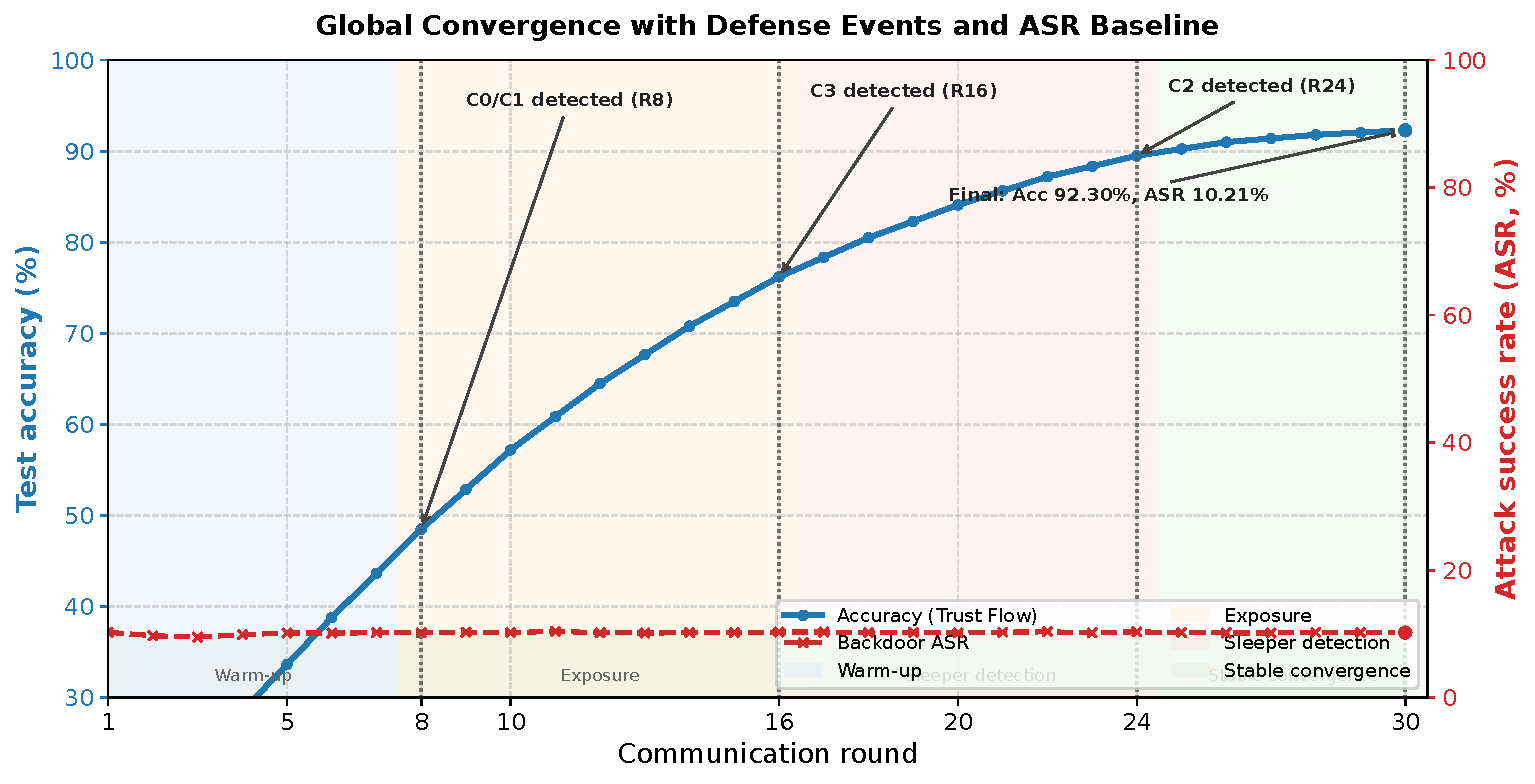
\includegraphics[width=\linewidth]{fig6_convergence_asr.pdf}
        \vspace{-3pt}
        {\scriptsize (a) 准确率与 ASR 收敛。}
    \end{minipage}\hfill
    \begin{minipage}{0.49\textwidth}
        \centering
        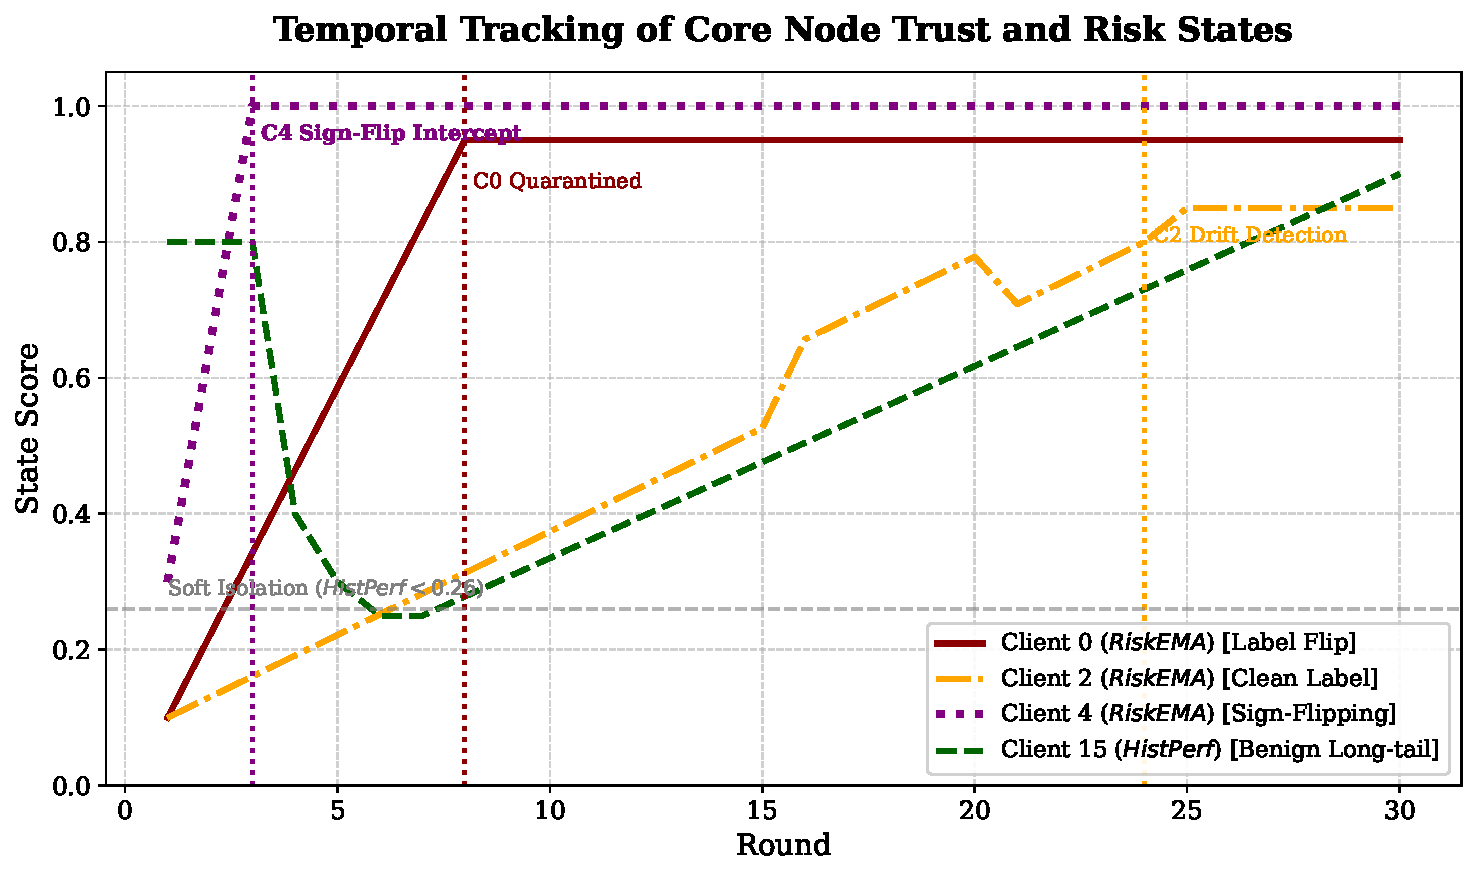
\includegraphics[width=\linewidth]{fig7_node_state_evolution.pdf}
        \vspace{-3pt}
        {\scriptsize (b) 节点信任与风险轨迹。}
    \end{minipage}
    \vspace{2pt}
    \begin{minipage}{0.57\textwidth}
        \centering
        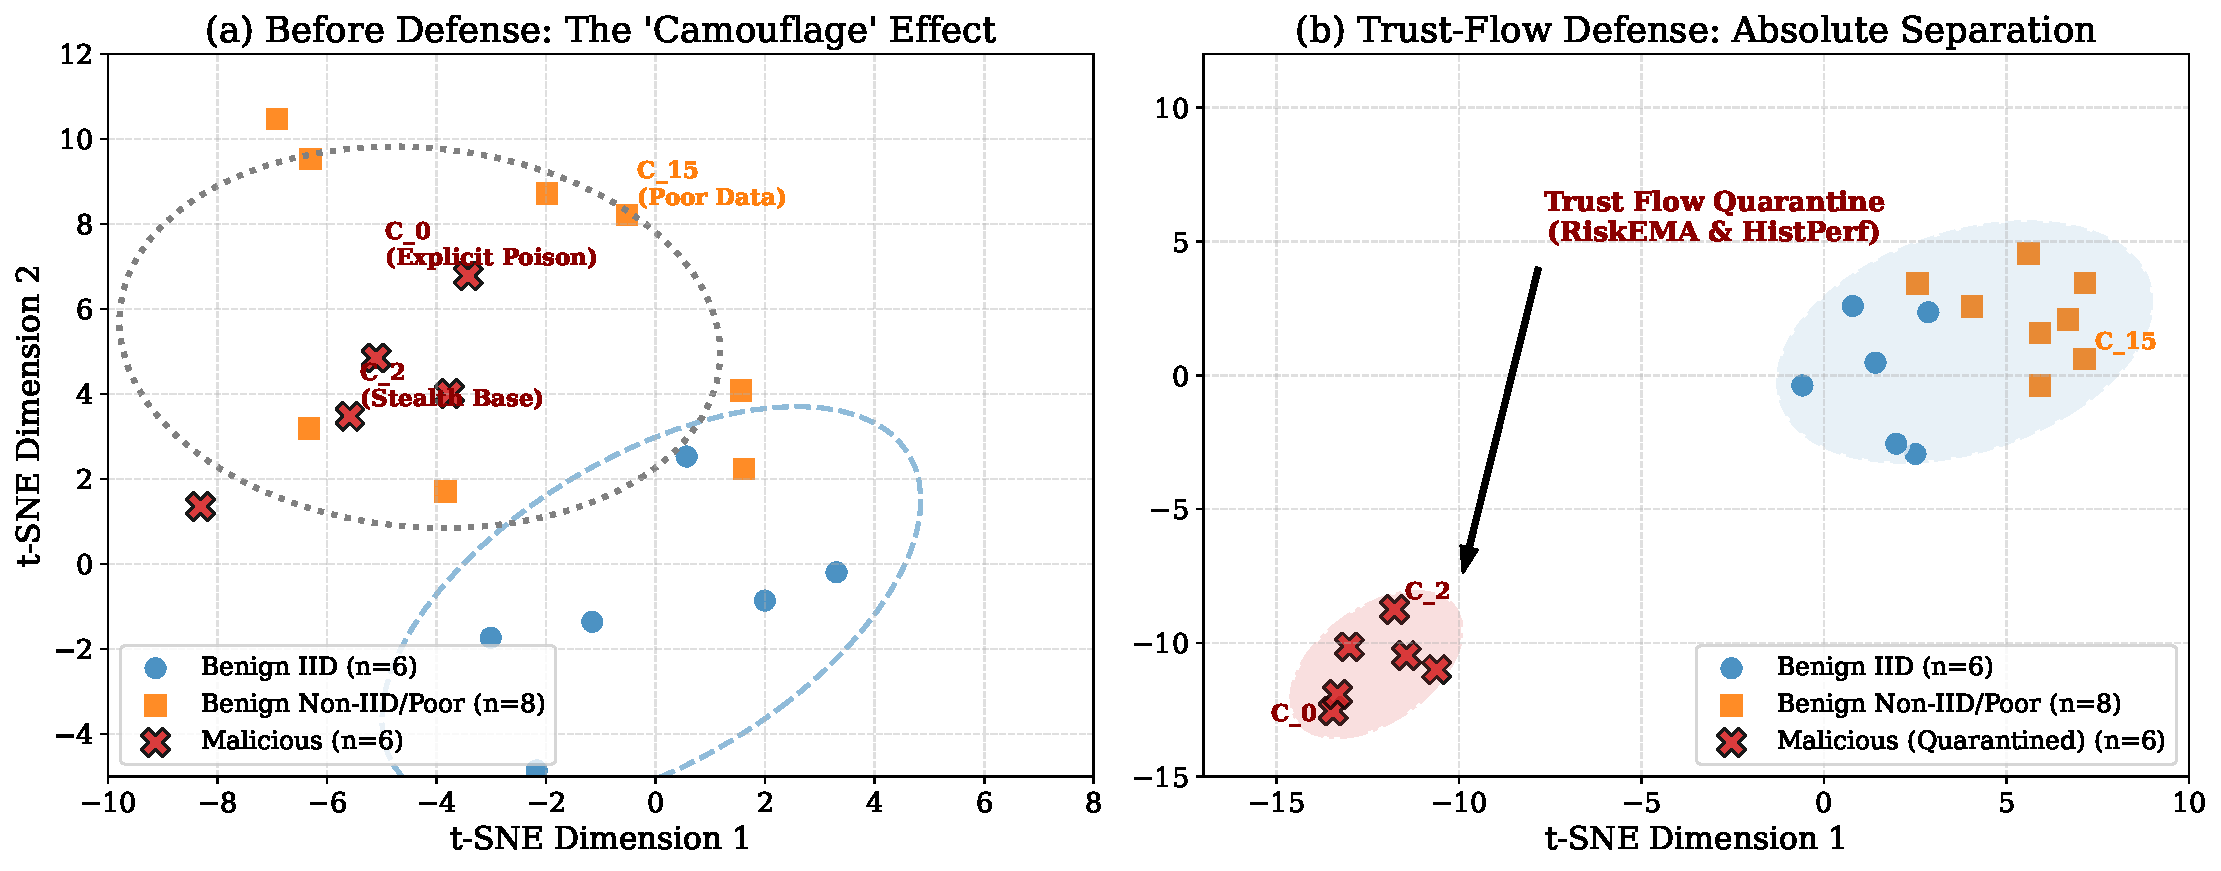
\includegraphics[width=\linewidth]{fig8_tsne_visualization.pdf}
        \vspace{-3pt}
        {\scriptsize (c) 防御前后 t-SNE 分离。}
    \end{minipage}
    \caption{混合攻击下的主要防御行为。}
    \label{fig:main_results}
\end{figure}

\begin{table}[t]
    \centering
    \begin{threeparttable}
        \caption{30\% 混合攻击与边界压力测试下的性能比较。}
        \label{tab:main_results}
        \scriptsize
        \setlength{\tabcolsep}{2pt}
        \begin{tabular*}{\textwidth}{@{\extracolsep{\fill}} p{2.55cm} p{2.85cm} c c c}
            \toprule
            方法/设置 & 核心机制 & Acc. & ASR & Perm. FPR \\
            \midrule
            FedAvg \cite{mcmahan2017fedavg} & 无防御 & $86.15\pm1.20$ & $92.34\pm5.10$ & N/A \\
            Krum \cite{blanchard2017krum} & 欧氏选择 & $64.20\pm2.80$ & $12.15\pm0.90$ & N/A \\
            Trimmed Mean \cite{yin2018byzantine} & 坐标截断 & $71.35\pm2.40$ & $38.60\pm4.20$ & N/A \\
            FLTrust \cite{cao2021fltrust} & 干净锚点加权 & $81.25\pm1.50$ & $15.42\pm1.10$ & N/A \\
            \textbf{Trust Flow} & 双流 + 分层门控 & $\mathbf{92.31\pm0.09}$ & $\mathbf{10.21\pm0.05}$ & $\mathbf{0.00}$ \\
            \midrule
            边界压力：50\% 恶意 & 10/20 恶意 & $91.81\pm0.10$ & $10.46\pm0.06$ & $0.00$ \\
            \bottomrule
        \end{tabular*}
        \begin{tablenotes}
            \scriptsize
            \item FPR 表示良性客户端的不可逆误封。临时 SUSPECT/QUARANTINE 状态是可恢复控制动作，并通过轨迹单独呈现。
        \end{tablenotes}
    \end{threeparttable}
\end{table}

在匹配的经典基线比较中，Krum、Trimmed Mean 与 FLTrust 以一定准确率代价降低了 ASR，Trust Flow 在相同协议下取得 92.31\% 的准确率和 10.21\% 的目标 ASR 宏平均值。上述结果仅描述本实验协议下的重复运行汇总，不构成普适性排序；DeepSight、FLAME、CrowdGuard、RoseAgg、FLPurifier、ShieldFL 与 RaSA 等近期方法需要本文未复现的攻击或隐私接口，因此未纳入直接比较。50\% 结果属于超出假设范围的压力测试，不能据此推导 Byzantine 理论边界。

\subsection{消融、敏感性与开销}

表~\ref{tab:ablation_overhead} 表明，单流信誉模型面临 FPR/TPR 权衡：激进阈值增加误封，保守阈值漏检潜伏攻击。仅使用 HistPerf 可以保护良性节点，却缺少短期攻击敏感性。双流设计在保持永久误封较低的同时获得较高召回。TrustReport 每次上传约增加 15 KB，服务器聚合与审查时间从每轮 2.10 s 增至 4.85 s；该服务器侧测量不包含端到端通信和厂商特定证明延迟，enclave 切换、内存压力和密码学聚合路径另行实测为每个准入客户端每轮约 11 ms。密码学 secure aggregation 不在本文系统边界内。

辅助安全路径实测结果表明，每个准入客户端每轮的 enclave 切换、内存压力和密码学聚合路径额外开销约为 11 ms；设备侧 TEE Quote 生成、签名和轻量监测另行实测为每个准入客户端每轮约 12--15 ms。上述辅助路径与服务器侧主要结果分开报告，因为主协议仍需检查单个客户端的证据。

\begin{table}[t]
    \centering
    \caption{消融与开销概要。}
    \label{tab:ablation_overhead}
    \scriptsize
    \setlength{\tabcolsep}{2pt}
    \begin{tabular*}{\textwidth}{@{\extracolsep{\fill}} p{2.1cm} p{4.45cm} c c}
        \toprule
        研究项 & 变体/架构 & FPR 或开销 & TPR / 时间 \\
        \midrule
        信誉 & 单流 EMA，激进 & 18.25\% FPR & 95.12\% TPR \\
        信誉 & 单流 EMA，保守 & 2.10\% FPR & 48.33\% TPR \\
        信誉 & HistPerf-only & 0.15\% FPR & 21.05\% TPR \\
        信誉 & \textbf{双流 Trust Flow} & \textbf{0.00\% FPR} & \textbf{100.00\% TPR} \\
        \midrule
        开销 & 标准 FedAvg & 额外 0 KB & 2.10 s 聚合 \\
        开销 & Trust Flow & $\sim$15 KB TrustReport & 4.85 s 含审查 \\
        \bottomrule
    \end{tabular*}
\end{table}

表~\ref{tab:ablation_overhead} 中 FPR/TPR 采用最终封禁口径。若将 SUSPECT 计为可逆风险复核状态，则恶意客户端逐轮覆盖率为 88.33\%，正常客户端复核触发率为 14.79\%，且不构成永久误杀。

图~\ref{fig:ablation_components} 和图~\ref{fig:alpha_sensitivity} 进一步分解了风险探针、权重重归一化和数据异构性的影响。干净参考结合浅层探针能够处理符号翻转和梯度缩放，但在梯度方向与良性更新共线时，干净标签后门仍较难识别。加入交叉熵与高层激活探针后，干净标签 ASR 降至 9.2\% 以下。重归一化同样重要：没有幸存者权重修正的分层门控会产生隐式学习率衰减，而完整 Trust Flow 能在 30 轮预算内收敛。在 Dirichlet $\alpha=0.1$ 下，Krum 与 FLTrust 明显退化，而 Trust Flow 仍保持接近 92\% 的准确率。

Dirichlet 扫描属于同一家族分布偏移测试：标签空间、模型、优化器和攻击协议保持不变，仅将浓度参数从弱异构调整到强异构。随着 $\alpha$ 降低，Krum 与 FLTrust 越来越容易排除合法漂移；Trust Flow 在所报告的扫描范围内对该变化较不敏感，因为内容证据与历史效用和瞬时风险共同整合。该结果是经验观察，不构成分布无关保证。融合参数 $\beta_{fusion}$ 控制干净参考支配群体一致性的强度，默认 $\beta_{fusion}=2.0$ 在观察结果中取得最好的 Acc/ASR 平衡。

开销分析将服务器侧 Trust Flow 处理与端到端部署成本分开。边缘侧附加约 15 KB 的 TrustReport；服务器执行参考构建、成对一致性审查、双流更新和按层裁剪，使聚合与审查时间从测试环境中的 2.10 s 增至 4.85 s。该测量报告的是服务器侧协议开销结果；辅助安全路径实测为每个准入客户端每轮约 11 ms，设备侧 TEE Quote 生成、签名和轻量监测另行实测为每个准入客户端每轮约 12--15 ms，端到端部署是否可接受仍取决于本文未测量的通信和厂商特定证明特性。

\begin{figure}[t]
    \centering
    \begin{minipage}{0.49\textwidth}
        \centering
        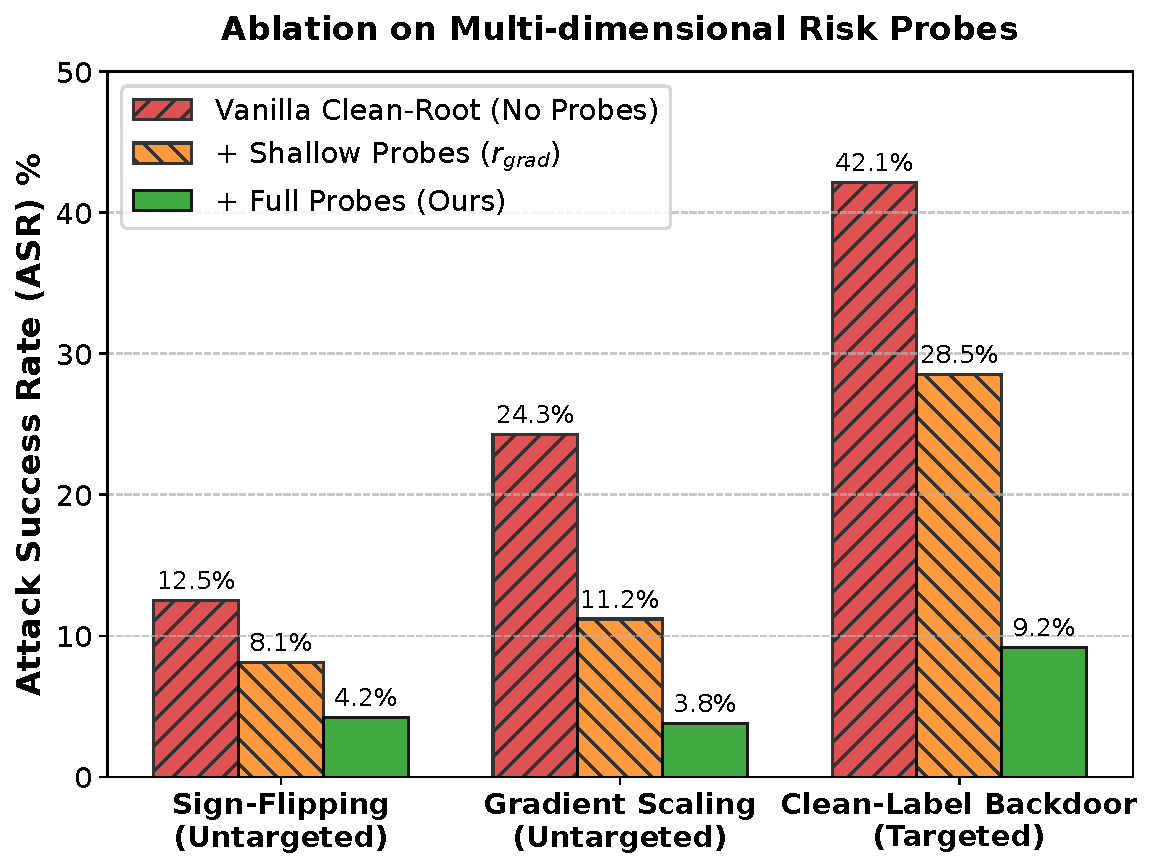
\includegraphics[width=\linewidth]{fig9_ablation_probes.pdf}
        \vspace{-3pt}
        {\scriptsize (a) 多维风险探针消融。}
    \end{minipage}\hfill
    \begin{minipage}{0.49\textwidth}
        \centering
        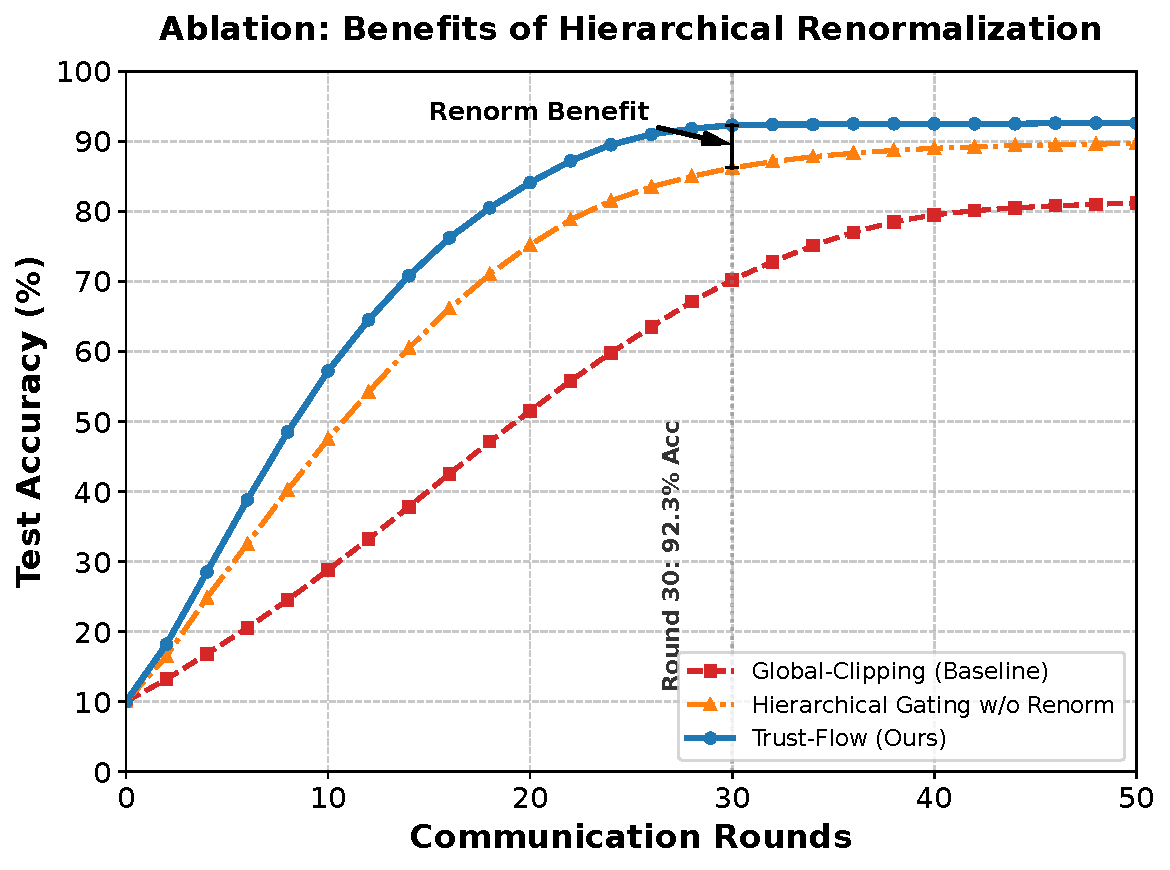
\includegraphics[width=\linewidth]{fig10_ablation_renorm.pdf}
        \vspace{-3pt}
        {\scriptsize (b) 权重重归一化效果。}
    \end{minipage}
    \caption{风险探针与重归一化的组件级消融。}
    \label{fig:ablation_components}
\end{figure}

\begin{figure}[t]
    \centering
    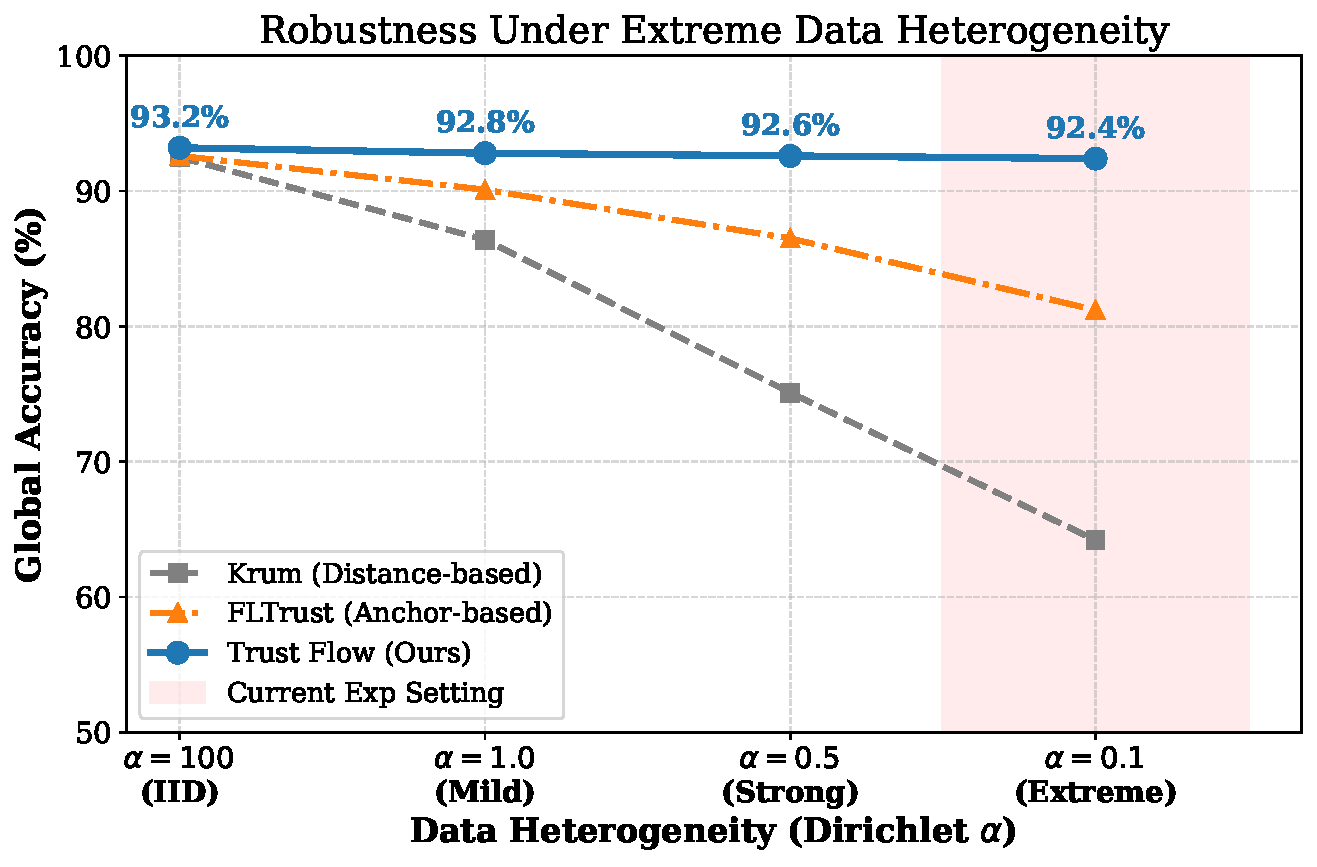
\includegraphics[width=0.76\textwidth]{fig11_alpha_sensitivity.pdf}
    \caption{不同数据异构度下的鲁棒性压力测试。}
    \label{fig:alpha_sensitivity}
\end{figure}

\section{讨论与结论}

Trust Flow 将执行准入、隐私感知统计检查、内容审查、时序信誉和分层聚合整合为统一的信任状态管线。其系统级贡献在于这些证据流的顺序与分离：执行证据控制准入，隐私感知检查提供有界数据证据，当前探针控制即时风险，历史效用控制可恢复保留，分层分数控制更新可贡献的位置。在所测试的 Intel 与 AMD TEE 支持配置上，该分离使永久封禁 FPR 保持接近零，同时对混合攻击保持较高召回。由此形成明确的保证边界：证明建立执行资格，云端内容与时序证据决定更新安全性。

本文评估的部署形态为服务器辅助的视觉联邦学习，具有小型可信参考划分及支持证明的客户端路径。对等参考分支将同一决策顺序扩展至不提供服务器 proxy 的部署，当前测量聚焦共同的参考初始化路径。微架构侧信道及厂商特定 enclave 资源争用位于威胁模型之外。探针面向视觉分类设计，开销分别报告服务器审查、辅助安全路径及设备侧证明组件，而非合并为单一端到端延迟。密码学 secure aggregation 不在主系统边界内，因为服务器需要检查逐客户端证据。该明确的部署形态界定信任流决策契约的适用范围，并为扩展到其他数据模态与部署条件提供基础。

\begingroup
\small
\begin{thebibliography}{99}
    \setlength{\itemsep}{0pt}
    \bibitem{kairouz2021flsurvey} Kairouz, P., McMahan, H.B., Avent, B., et al.: Advances and open problems in federated learning. Foundations and Trends in Machine Learning 14(1--2), 1--210 (2021). \url{https://doi.org/10.1561/2200000083}
    \bibitem{mcmahan2017fedavg} McMahan, B., Moore, E., Ramage, D., Hampson, S., Aguera y Arcas, B.: Communication-efficient learning of deep networks from decentralized data. In: Proceedings of the 20th International Conference on Artificial Intelligence and Statistics, PMLR 54, pp. 1273--1282 (2017). \url{https://proceedings.mlr.press/v54/mcmahan17a.html}
    \bibitem{blanchard2017krum} Blanchard, P., El Mhamdi, E.M., Guerraoui, R., Stainer, J.: Machine learning with adversaries: Byzantine tolerant gradient descent. In: Advances in Neural Information Processing Systems 30 (2017). \href{https://papers.nips.cc/paper/6617-machine-learning-with-adversaries-byzantine-tolerant-gradient-descent}{NeurIPS paper page}
    \bibitem{yin2018byzantine} Yin, D., Chen, Y., Ramchandran, K., Bartlett, P.: Byzantine-robust distributed learning: Towards optimal statistical rates. In: Proceedings of the 35th International Conference on Machine Learning, PMLR 80, pp. 5650--5659 (2018). \url{https://proceedings.mlr.press/v80/yin18a.html}
    \bibitem{cao2021fltrust} Cao, X., Fang, M., Liu, J., Gong, N.Z.: FLTrust: Byzantine-robust federated learning via trust bootstrapping. In: Proceedings 2021 Network and Distributed System Security Symposium (NDSS) (2021). \url{https://doi.org/10.14722/ndss.2021.24434}
    \bibitem{fung2020foolsgold} Fung, C., Yoon, C.J.M., Beschastnikh, I.: The limitations of federated learning in Sybil settings. In: 23rd International Symposium on Research in Attacks, Intrusions and Defenses (RAID 2020), pp. 301--316. USENIX Association (2020). \url{https://www.usenix.org/conference/raid2020/presentation/fung}
    \bibitem{wang2025rasa} Wang, L., Huang, M., Zhang, Z., Li, M., Wang, J., Gai, K.: RaSA: Robust and adaptive secure aggregation for edge-assisted hierarchical federated learning. IEEE Transactions on Information Forensics and Security 20, 4280--4295 (2025). \url{https://doi.org/10.1109/TIFS.2025.3559411}
    \bibitem{fldetector2022} Zhang, Z., Cao, X., Jia, J., Gong, N.Z.: FLDetector: Defending federated learning against model poisoning attacks via detecting malicious clients. In: Proceedings of the 28th ACM SIGKDD Conference on Knowledge Discovery and Data Mining, pp. 2545--2555 (2022). \url{https://doi.org/10.1145/3534678.3539231}
    \bibitem{deepsight2022} Rieger, P., Nguyen, T.D., Miettinen, M., Sadeghi, A.R.: DeepSight: Mitigating backdoor attacks in federated learning through deep model inspection. In: Network and Distributed System Security Symposium (NDSS) (2022). \url{https://doi.org/10.14722/ndss.2022.23156}
    \bibitem{flame2022} Nguyen, T.D., Rieger, P., Chen, H., et al.: FLAME: Taming backdoors in federated learning. In: 31st USENIX Security Symposium, pp. 1415--1432 (2022). \url{https://www.usenix.org/conference/usenixsecurity22/presentation/nguyen}
    \bibitem{crowdguard2024} Rieger, P., Krau{\ss}, T., Miettinen, M., Dmitrienko, A., Sadeghi, A.R.: CrowdGuard: Federated backdoor detection in federated learning. In: Network and Distributed System Security Symposium (NDSS) (2024). \url{https://doi.org/10.14722/ndss.2024.23233}
    \bibitem{flpurifier} Zhang, J., Zhu, C., Sun, X., Ge, C., Chen, B., Susilo, W., Yu, S.: FLPurifier: Backdoor defense in federated learning via decoupled contrastive training. IEEE Transactions on Information Forensics and Security 19, 4752--4766 (2024). \url{https://doi.org/10.1109/TIFS.2024.3384846}
    \bibitem{roseagg} Yang, H., Xi, W., Shen, Y., Wu, C., Zhao, J.: RoseAgg: Robust defense against targeted collusion attacks in federated learning. IEEE Transactions on Information Forensics and Security 19, 2951--2966 (2024). \url{https://doi.org/10.1109/TIFS.2024.3352415}
    \bibitem{shieldfl} Ma, Z., Ma, J., Miao, Y., Li, Y., Deng, R.H.: ShieldFL: Mitigating model poisoning attacks in privacy-preserving federated learning. IEEE Transactions on Information Forensics and Security 17, 1639--1654 (2022). \url{https://doi.org/10.1109/TIFS.2022.3169918}
    \bibitem{zhang2025rppfl} Zhang, X., Chen, Z., Chen, G., Feng, X., Shen, Q., Wu, Z.: RPPFL: Robust and privacy-preserving federated learning via trusted execution environments. In: ICASSP 2025 - 2025 IEEE International Conference on Acoustics, Speech and Signal Processing, pp. 1--5 (2025). \url{https://doi.org/10.1109/ICASSP49660.2025.10889398}
    \bibitem{r1_tee_integrity} Chen, Y., Luo, F., Li, T., Xiang, T., Liu, Z., Li, J.: A training-integrity privacy-preserving federated learning scheme with trusted execution environment. Information Sciences 522, 69--79 (2020). \url{https://doi.org/10.1016/j.ins.2020.02.037}
    \bibitem{r5_tee_mitigating} Queyrut, S., Schiavoni, V., Felber, P.: Mitigating adversarial attacks in federated learning with trusted execution environments. In: 2023 IEEE 43rd International Conference on Distributed Computing Systems (ICDCS), pp. 626--637 (2023). \url{https://doi.org/10.1109/ICDCS57875.2023.00069}
    \bibitem{xu2021distributed} Xu, T., Zhu, K., Andrzejak, A., Zhang, L.: Distributed learning in trusted execution environment: A case study of federated learning in SGX. In: 2021 7th IEEE International Conference on Network Intelligence and Digital Content (IC-NIDC), pp. 450--454 (2021). \url{https://doi.org/10.1109/IC-NIDC54101.2021.9660433}
    \bibitem{lu2025tmt} Lu, Z., Wang, L., Zhang, Z., Huang, M., Wang, J., Li, M.: TMT-FL: Enabling trustworthy model training of federated learning with malicious participants. IEEE Transactions on Dependable and Secure Computing 22(3), 2723--2740 (2025). \url{https://doi.org/10.1109/TDSC.2024.3521377}

    \bibitem{bagdasaryan2020backdoor} Bagdasaryan, E., Veit, A., Hua, Y., Estrin, D., Shmatikov, V.: How To Backdoor Federated Learning. In: Proceedings of the Twenty Third International Conference on Artificial Intelligence and Statistics, PMLR 108, pp. 2938--2948 (2020). \url{https://proceedings.mlr.press/v108/bagdasaryan20a.html}
    \bibitem{wang2019neuralcleanse} Wang, B., Yao, Y., Shan, S., Li, H., Viswanath, B., Zheng, H., Zhao, B.Y.: Neural Cleanse: Identifying and mitigating backdoor attacks in neural networks. In: 2019 IEEE Symposium on Security and Privacy (SP), pp. 707--723 (2019). \url{https://doi.org/10.1109/SP.2019.00031}

\end{thebibliography}
\endgroup

\end{document}
